\section{PHƯƠNG TRÌNH MẶT PHẲNG}
\subsection{LÝ THUYẾT CẦN NHỚ}
\subsubsection{Vec tơ pháp tuyến của mặt phẳng}
\vspace{-0.3cm}
\begin{itemize}
	\immini{\item [\iconMT] \indam{Định nghĩa:} Véc tơ pháp tuyến $\vec{n}$ của mặt phẳng $(P)$ là những véc tơ khác $\vec{0}$ và có giá vuông góc với $(P)$. 
		\item [\iconMT] \indam{Chú ý:} 
		\begin{boxdn}
			 Nếu $\vec{n}$ và $\vec{n'}$ cùng là véc tơ pháp tuyến của $(P)$ thì $\vec{n'} = k \cdot \vec{n}$ (tọa độ tỉ lệ nhau).
		\end{boxdn}
	}{\vspace{0.5cm}\hspace{1cm}
		\begin{tikzpicture}[scale=0.8, line join=round, line cap=round,>=stealth]
			\tkzDefPoints{0/0/A,4/0/B,5/2/C}
			\coordinate (D) at ($(A)+(C)-(B)$);
			\tkzDrawPolygon(A,B,C,D)
			\tkzMarkAngles[size=0.7cm,arc=l](B,A,D)
			\tkzLabelAngles[pos=0.5,rotate=10](B,A,D){\scriptsize$P$}
			\draw[->] (2,1)--(2,2.5)node[right]{\scriptsize$\vec{n}$};
			\draw[->] (3,1.5)--(3,3)node[right]{\scriptsize$\vec{n'}$};
	\end{tikzpicture}}
\end{itemize}

\subsubsection{Cặp vec-tơ chỉ phương của mặt phẳng}
\vspace{-0.3cm}
\begin{itemize}
	\item [\iconMT] \indam{Định nghĩa:} Trong không gian $Oxyz$, cho hai véc-tơ $\vec u$, $\vec v$ được gọi là cặp véc-tơ chỉ phương của mặt phẳng $(P)$ nếu chúng không cùng phương và có giá nằm trong hoặc song song với mặt phẳng $(P)$.
	\item [\iconMT] \indam{Chú ý:} 
	\begin{boxdn}
\immini{		\begin{itemize}
			\item [$\bullet$] Cho hai vectơ $\vec u = (a; b; c)$ và $\vec v = (a'; b'; c')$. Khi đó 
			$$\vec n = (bc' - b'c;ca' - c'a; ab' - a'b)$$
			vuông góc với cả hai vectơ $\vec u$ và $\vec v$, được gọi là tích có hướng của $\vec u$ và $\vec v$, ký hiệu là $[\vec u, \vec v]$.
			\item [$\bullet$] Nếu $\vec u$, $\vec v$ là cặp véc-tơ chỉ phương của $(P)$ thì $[\vec u,\vec v]$ là một véc-tơ pháp tuyến của $(P)$.
		\end{itemize}}{
	\begin{tikzpicture}[>=stealth, line join=round, line cap = round,scale=0.8]
	\def\d{4}
	\def\r{3}
	\path (0:0) coordinate (B)
	++(0:\d) coordinate (C)
	++(50:\r) coordinate (D)
	($(B)+(D)-(C)$) coordinate (A)
	(2.5,2) coordinate (M)
	(3.5,2) coordinate (N)
	(3.,1.6) coordinate (P)
	;
	\draw[->] (M)--($(M)+(-130:1.5)$) node[pos=0.4,left] {$\vec u$};
	\draw[->] (N)--($(N)+(0:1.8)$) node[pos=0.4,below] {$\vec v$};
	\draw[->] (P)--($(P)+(90:1.8)$) node[pos=0.9,right] {${[\vec u,\vec v]}$};
	\draw (A)--(B)--(C)--(D)--cycle;
	\begin{scope}
		\clip (A)--(B)--(C);
		\draw[opacity=0.7] (B) circle(0.8cm)node[black,shift={(25:4mm)}]{$P$};
	\end{scope}
	%		\foreach \x/ \goc in {A/180,B/180,C/0,D/0} 
	%		\fill (\x) circle (1pt) ($(\x)+(\goc:3mm)$) node {$\x$};
\end{tikzpicture}}
	\end{boxdn}

\end{itemize}
\subsubsection{Phương trình tổng quát của mặt phẳng}
\begin{itemize}
	\item [\iconMT] \indam{Công thức:} Mặt phẳng $(P)$ đi qua điểm $M(x_0;y_0;z_0)$ và nhận $\vec{n}=(a;b;c)$ làm véc tơ pháp tuyến có phương trình là 
	\boxminit{$a(x-x_0)+b(y-y_0)+c(z-z_0)=0$}
	Thu gọn ta được dạng $ax+by+cz+d=0$.
	\item [\iconMT] \indam{Chú ý:}
	\begin{boxdn}
		\begin{itemize}
			\item [\ding{172}] Phương trình các mặt phẳng tọa độ: 
			\begin{listEX}[2]
				\item [$\bullet$] $(Oxy) \colon z=0$.
				\item [$\bullet$] $(Oxz) \colon y=0$.
				\item [$\bullet$] $(Oyz) \colon x=0$.
			\end{listEX}
			\item [\ding{173}] Phương trình mặt phẳng $(\alpha)$ song song với mặt phẳng tọa độ: 
			\begin{listEX}[2]
				\item [$\bullet$] $(\alpha) \parallel (Oxy) \Rightarrow z=a \quad a \ne 0$.
				\item [$\bullet$] $(\alpha) \parallel (Oxz) \Rightarrow y=b \quad b \ne 0 $.
				\item [$\bullet$] $(\alpha) \parallel (Oyz) \Rightarrow x=c \quad c \ne 0$.
			\end{listEX}
		\end{itemize}
	\end{boxdn}
\end{itemize}

\subsubsection{Vị trị tương đối giữa hai mặt phẳng}
\begin{itemize}
	\item [] Cho hai mặt phẳng $(P) \colon a_1x + b_1y + c_1z + d_1=0$ và $(Q) \colon a_2x + b_2y + c_2z + d_2=0$. \\
	Gọi $\vec{n_1}=(a_1;b_1;c_1)$, $\vec{n_2}=(a_2;b_2;c_2)$ lần lượt là véc tơ pháp tuyến của $(P)$ và $(Q)$.\\
	\begin{boxdn}
		\begin{listEX}[1]
			\item [\ding{172}] Nếu $\heva{&\vec{n_1}= k \cdot \vec{n_2}\\& d_1 =k\cdot d_2}$ thì $(P)$ trùng $(Q)$.
			\item [\ding{173}] Nếu $\heva{&\vec{n_1}= k \cdot \vec{n_2}\\& d_1 \ne k\cdot d_2}$ thì $(P)$ song song $(Q)$.
			\item [\ding{174}] Nếu $\vec{n_1}$ không cùng phương với $\vec{n_2}$ thì $(P)$ cắt $(Q)$.
			\item [\ding{175}] Nếu $\vec{n_1} \perp \vec{n_2}$ hay $a_1a_2+b_1b_2+c_1c_2=0$ thì $(P) \perp (Q)$.
		\end{listEX}
	\end{boxdn}  
\end{itemize}

\subsubsection{Khoảng cách từ một điểm đến mặt phẳng}
\vspace{-0.4cm}
\begin{itemize}
	\immini{\item [\iconMT] \indam{Định nghĩa:} Cho điểm $M(x_0;y_0;z_0)$ và mặt phẳng $(P) \colon ax+by+cz+d=0$. Gọi $H$ là hình chiếu vuông góc của điểm $M$ lên mặt phẳng $(P)$. Khi đó độ dài đoạn $MH$ được gọi là khoảng cách từ điểm $M$ đến $(P)$. Kí hiệu $\mathrm{d}\left(M,(P) \right)$.
		\item [\iconMT] \indam{Công thức tính:}
		\boxminit{$\mathrm{d}\left(M,(P) \right)=\dfrac{\bigg|ax_0+by_0+cz_0+d\bigg|}{\sqrt{a^2+b^2+c^2}}$}
	}{\vspace{0.5cm} \hspace{1cm}
		\begin{tikzpicture}[scale=0.8, line join=round, line cap=round]
			\tkzDefPoints{0/0/A,4/0/B,5/2/C}
			\coordinate (D) at ($(A)+(C)-(B)$);
			\tkzDrawPolygon(A,B,C,D)
			\tkzMarkAngles[size=0.7cm,arc=l](B,A,D)
			\tkzLabelAngles[pos=0.5,rotate=10](B,A,D){$P$}
			\draw (2,1)node[right]{$H$}--(2,3)node[above]{$M$};
			\draw[fill=black] (2,1) circle(1.5pt) (2,3) circle(1.5pt);
	\end{tikzpicture}}
	\item [\iconMT] \indam{Chú ý} 
	\begin{listEX}[1]
		\item [\ding{172}] $\mathrm{d}\left(M,(Oxy) \right)=\big|z_M\big|$.
		\item [\ding{173}]  $\mathrm{d}\left(M,(Oxz) \right)=\big|y_M\big|$.
		\item [\ding{174}]  $\mathrm{d}\left(M,(Oyz) \right)=\big|x_M\big|$.
		\item [\ding{175}] Cho hai mặt phẳng $(P) \colon ax + by + cz + d_1=0$ và $(Q) \colon ax + by + cz + d_2=0$ song song nhau. 
		Khi đó
		\boxminit{$\mathrm{d}\left((P),(Q) \right)=\dfrac{\bigg|d_1-d_2\bigg|}{\sqrt{a^2+b^2+c^2}}$}
	\end{listEX}
\end{itemize}

\subsection{PHÂN LOẠI, PHƯƠNG PHÁP GIẢI TOÁN}
\begin{dang}{Xác định véc tơ pháp tuyến và điểm thuộc mặt phẳng}
	Cho mặt phẳng $(\alpha)$.
	\begin{itemize}
		\item  [\ding{172}] Nếu véctơ $\overrightarrow{n} \ne \overrightarrow{0}$ và có giá vuông góc với $(\alpha)$ thì $\overrightarrow{n}$ là một véctơ pháp tuyến của $(\alpha)$.
		\item  [\ding{173}] Nếu hai véctơ $\overrightarrow{a}, \overrightarrow{b}$ không cùng phương, có giá song song hoặc nằm trong $(\alpha)$ thì $\overrightarrow{a}, \overrightarrow{b}$ được gọi là cặp véctơ chỉ phương của $(\alpha)$. Khi đó, nếu $\vec{a}=(a_1;a_2;a_3)$, $\vec{b}=(b_1;b_2;b_3)$ thì
		$$\vec{n}= [\vec{a}, \vec{b}]=\left(\left|\begin{array}{ll}a_2 & a_3 \\ b_2 & b_3\end{array}\right| ;\left|\begin{array}{ll}a_3 & a_1 \\ b_3 & b_1\end{array}\right| ;\left|\begin{array}{ll}a_1 & a_2 \\ b_1 & b_2\end{array}\right|\right)$$ là một véc-tơ pháp tuyến của mặt phẳng $(P)$.
		\item [\ding{174}] Nếu $(\alpha) \colon ax + by + cz + d = 0$ thì $(\alpha)$ có một véc tơ pháp tuyến là $\vec{n}=(a;b;c)$.
	\end{itemize}
\end{dang}
\boxmini{BÀI TẬP TỰ LUẬN}

\begin{vd}
	\immini{Cho hình lập phương $ABCD.A'B'C'D'$. 
		\begin{tasks}
			\task Xác định véc tơ pháp tuyến của các mặt phẳng $(ABCD)$,  $(ABB'A')$,  $(ACC'A')$,  $(ADD'A')$.
			\task Chứng minh $\vec{AB'}$ là một véc tơ pháp tuyến của $(BCD'A')$.
		\end{tasks}
	}{
	\begin{tikzpicture}[scale=0.8, font=\footnotesize, line join=round, line cap=round, >=stealth]
		\def\bc{4} % cạnh BC
		\def\ba{2} % cạnh BA
		\def\h{3} % đường cao
		\def\gocB{35} % góc B của đáy
		\coordinate[label=below left:$B$] (B) at (0,0);
		\coordinate[label=above left:$A$] (A) at (\gocB:\ba);
		\coordinate[label=below:$C$] (C) at (\bc,0);
		\coordinate[label=right:$D$] (D) at ($(C)-(B)+(A)$);
		\coordinate[label=above left:$A'$] (A') at ($(A)+(90:\h)$);
		\coordinate[label=left:$B'$] (B') at ($(B)-(A)+(A')$);
		\coordinate[label=below right:$C'$] (C') at ($(C)-(A)+(A')$);
		\coordinate[label=right:$D'$] (D') at ($(D)-(A)+(A')$);
		\draw (B')--(B)--(C)--(D)--(D')--(A')--(B')--(C')--(D') (C)--(C');
		\draw[dashed] (A')--(A)--(D) (A)--(B);
		\foreach \diem in {A,B,C,D,A',B',C',D'}	\fill (\diem)circle(1.5pt);
\end{tikzpicture}}
	\loigiai{a) Véc tơ pháp tuyến của $(ABCD)$ là $\vec{AA'}, \vec{BB'}, \vec{CC'}, \vec{DD'}$.\\
	Véc tơ pháp tuyến của $(ABB'A')$ là $\vec{AD}, \vec{BC}, \vec{B'C'}, \vec{A'D'}$.\\
	Véc tơ pháp tuyến của $(ACC'A')$ là $\vec{BD}, \vec{B'D'}$.\\
	Véc tơ pháp tuyến của $(ADD'A')$ là $\vec{AB}, \vec{DC}, \vec{D'C'}, \vec{A'B'}$.\\\\
	b) Chứng minh: $\vec{AB'}\perp\vec{A'B}$ và $\vec{AB'}\perp\vec{BC}$.\\
	Suy ra: $\vec{AB'}\perp(BCD'A')$.}
\end{vd}

\dongcham{2}
\begin{vd}
	Cho mặt phẳng $(P): 2x-3y+4z+5=0$. Hãy chỉ ra một vectơ pháp tuyến của $(P)$ và hai điểm thuộc $(P)$. 

	\loigiai{Véc-tơ $\overrightarrow{n}=(2;-3;4) $ là một véc-tơ pháp tuyến của mặt phẳng $(P)$.\\ 
	Điểm $(1;1-1)$ và $(0;3;1)$ thuộc $(P)$.	
	}
\end{vd}
\dongcham{2}

\begin{vd}
	Cho $(P)$ là mặt phẳng trung trực của $MN$ với $M(1;-2;3)$, $N(1;4;1)$. Hãy chỉ ra một vectơ pháp tuyến của $(P)$ và một điểm thuộc $(P)$.
	\loigiai{
		Mặt phẳng trung trực của $MN$ đi qua trung điểm của $MN$ và vuông góc với $MN$.\\
		Vậy $\vec{MN}=(0; 6; -2)$ là một vectơ pháp tuyến của mặt phẳng $(P)$ và điểm $(1;1;2)$ thuộc $(P)$.
	}
\end{vd}
\dongcham{3}
\begin{vd}
	Chỉ ra một vectơ pháp tuyến của mặt phẳng $(\alpha)$ biết $(\alpha)$ đi qua
	\begin{listEX}[1]
		\item $A(-1; 3; 5)$, $B(3;2;-2)$ và $C(0; 3; 0)$;
		\item $M(0; 3; 1)$, $N(-3;2;5)$ và $P(-2; 0; 0)$.
	\end{listEX}
	\loigiai{
		\begin{listEX}[1]
			\item 	Ta có $\vec{AB} = (4; -1;-7)$, $\vec{AC} = (1; 0; -5)$.\\
			Xét vectơ $\vec{n}=[\vec{AB}, \vec{AC}] = \left(\left|\begin{array}{cc}-1 & -7 \\ 0 & -5\end{array}\right| ;\left|\begin{array}{cc}-7 & 4 \\ -5 & 1\end{array}\right| ;\left|\begin{array}{cc}4 & -1 \\ 1 & 0\end{array}\right|\right)=(5 ; 13 ; 1)$.\\
			Vậy $\vec{n} = (5 ; 13 ; 1)$ là một vectơ pháp tuyến của mặt phẳng $(\alpha)$.
			\item Ta có $\vec{MN} = (-3; -1;4)$, $\vec{MP} = (-2; -3; -1)$.\\
			Xét vectơ $\vec{n}=[\vec{MN}, \vec{MP}] = \left(\left|\begin{array}{cc}-1 & 4 \\ -3 & -1\end{array}\right| ;\left|\begin{array}{cc}4 & -3 \\ -1 & -2\end{array}\right| ;\left|\begin{array}{cc}-3 & -1 \\ -2 & -3\end{array}\right|\right)=(13; -11; 7)$.\\
			Vậy $\vec{n} = (13 ; -11 ; 7)$ là một vectơ pháp tuyến của mặt phẳng $(\alpha)$.
		\end{listEX}
	}
\end{vd}
\dongcham{6}


\begin{vd}
Cho tứ diện $ABCD$ có các đỉnh là $A(5 ; 1 ; 3)$, $B(1 ; 6 ; 2)$, $C(5 ; 0 ; 4)$ và $D(4 ; 0 ; 6)$. Gọi $(\alpha)$ là mặt phẳng chứa cạnh $AB$ và song song với cạnh $CD$. Hãy tìm một điểm thuộc $(\alpha)$ và một véc tơ pháp tuyến của $(\alpha)$.
	\loigiai{
		Ta có $\overrightarrow{AB}=(-4 ; 5 ;-1)$, $\overrightarrow{CD}=(-1 ; 0 ; 2)$ nên $\overrightarrow{AB}, \overrightarrow{CD}$ không cùng phương.\\
		Mà giá của $\overrightarrow{AB}$ nằm trong mặt phẳng $(\alpha)$ và giá của $\overrightarrow{CD}$ song song với mặt phẳng $(\alpha)$ nên $\overrightarrow{AB}$, $\overrightarrow{CD}$ là một cặp véc-tơ chỉ phương của mặt phẳng $(\alpha)$.
		Vậy một véc-tơ pháp tuyến của $(\alpha)$ là
		$$
		\begin{aligned}
			\vec{n}=\left[\overrightarrow{AB}, \overrightarrow{CD}\right]&=
			\left(\left|\begin{array}{cc}
				5 & -1 \\
				0 & 2
			\end{array}\right| ;
			\left|\begin{array}{cc}
				-1 & -4 \\
				2 & -1
			\end{array}\right| ;
			\left|\begin{array}{cc}
				-4 & 5 \\
				-1 & 0
			\end{array}\right|\right) \\
			&=\left(5 \cdot 2-0 \cdot(-1) ; (-1)\cdot (-1) - 2 \cdot (-4) ; (-4) \cdot 0-5 \cdot (-1)\right) \\
			&=(10 ; 9 ; 5).
		\end{aligned}
		$$
	}
\end{vd}
\dongcham{4}
\boxmini{BÀI TẬP TRẮC NGHIỆM}
\setcounter{ex}{0}

\begin{ex}
	Cho mặt phẳng $(\alpha) \colon 2x-y+3z-2=0$. Điểm nào sau đây thuộc mặt phẳng $(\alpha)$?
	\choice
	{$A(1;-3;1)$}
	{\True $B(2;-1;-1)$}
	{$C(2;-1;1)$}
	{$D(1;2;3)$}
	\loigiai{
	Thay tọa độ các điểm vào phương trình $(\alpha)$, tọa độ $B(2;-1;-1)$ thỏa mãn.}
\end{ex}
\cham{1}
\begin{ex}%[2H3Y2-7]
	Cho mặt phẳng $(\alpha) \colon x+y+z-6=0$. Điểm nào dưới đây \textbf{không} thuộc $(\alpha)$?
	\choice
	{\True $M(1;-1;1)$}
	{$N(2;2;2)$}
	{$P(1;2;3)$}
	{$Q(3;3;0)$}
	\loigiai
	{
		Ta có $1-1+1-6=-5 \neq 0$ nên $M(1;-1;1)$ không thuộc $(\alpha)$.
	}
\end{ex}
\cham{1}
\begin{ex}
	Cho $(\alpha)$ vuông góc với giá của $\vec{a}=(2;-1;3)$. Vectơ nào dưới đây là vectơ pháp tuyến của $(\alpha)$?
	\choice
	{$\vec{n_1}=(-2;1;3)$}
	{\True $\vec{n_2}=(-2;1;-3)$}
	{$\vec{n_3}=(4;2;6)$}
	{$\vec{n_4}=(4;-2;-6)$}
	\loigiai{
		$(\alpha)$ vuông góc với giá của $\vec{a}=(2;-1;3)$ nên $\vec{a}$ là một vectơ pháp tuyến của $(\alpha)$.\\
		Do đó $\vec{n_2}=-\vec{a}$ cũng là một vectơ pháp tuyến của $(\alpha)$.
	}
\end{ex}
\cham{1}
\begin{ex}%[2H3B2-2]
	Vec-tơ nào sau đây \textbf{không} phải là vec-tơ pháp tuyến của mặt phẳng $(P):x+3y-5z+2=0$.
	\choice
	{$\overrightarrow{n}_1=(-1;-3;5)$}
	{\True $\overrightarrow{n}_2=(-2;-6;-10)$}
	{$\overrightarrow{n}_3=(-3;-9;15)$}
	{$\overrightarrow{n}_4=(2;6;-10)$}
	\loigiai{Mặt phẳng $(P)$ nhận vec-tơ $\overrightarrow{a}=(1;3;-5)$ làm vec-tơ pháp tuyến.\\
		Xét $\overrightarrow{n}_2=(-2;-6;-10)$ có $\dfrac{-2}{1}=\dfrac{-6}{3}\ne\dfrac{-10}{-5}$ nên $\overrightarrow{n}_2$ không cùng phương với $\overrightarrow{a}$.\\
		Suy ra $\overrightarrow{n}_2$ không là vec-tơ pháp tuyến của $(P)$.}
\end{ex}
\cham{1}
\begin{ex}
	Trong không gian  $Oxyz$, mặt phẳng tọa độ $(Oxy)$ có một véc-tơ pháp tuyến là
	\choice
	{$\overrightarrow{n}=(0;1;0)$}
	{\True $\overrightarrow{n}=(0;0;1)$}
	{$\overrightarrow{n}=(1;0;0)$}
	{$\overrightarrow{n}=(1;1;0)$}
	\loigiai{
		Mặt phẳng tọa độ $(Oxy)\colon x=0\Rightarrow$ 1 véc-tơ pháp tuyến là $\overrightarrow{n}=(0;0;1)$.}
\end{ex}
\cham{1}
\begin{ex}
	Trong không gian $Oxyz$, cho điểm $A(4;-3;7)$ và $B(2;1;3)$. Một véc tơ pháp tuyến của mặt phẳng trung trực của đoạn $AB$ là
	\choice
	{\True $\vec{n}=(1;-2;2)$}
	{$\vec{n}=(2;4;4)$}
	{$\vec{n}=(6;-2;10)$}
	{$\vec{n}=(-2;-4;4)$}
	\loigiai{
		Ta có $\overrightarrow{AB}(-2;4;-4)$ cùng phương với  $\vec{n}=(1;-2;2)$. Suy ra  $\vec{n}=(1;-2;2)$ là một véc tơ pháp tuyến.
	}
\end{ex}
\cham{1}
\begin{ex}%[HK1 - Chuyên Huỳnh Mẫn Đạt - Kiên Giang - 20-21]%[Phan Quốc Trí-EX5]%[2H3B2-2]%
	Trong không gian $Oxyz$, $(P)$ là mặt phẳng trung trực của đoạn $AB$, biết $A(1;3;0)$, $B(-2;1;-1)$. Véc-tơ nào sau đây là véc-tơ pháp tuyến của $(P)$?
	\choice
	{$\overrightarrow{n}_4=(3;-2;-1)$}
	{$\overrightarrow{n}_2=(-3;2;-1)$}
	{$\overrightarrow{n}_3=(-3;4;1)$}
	{\True $\overrightarrow{n}_1=(3;2;1)$}
	\loigiai{
		Mặt phẳng $(P)$ có véc-tơ pháp tuyến là  $\overrightarrow{BA}= (3;2;1)$.
	}
\end{ex}
\cham{1}
\begin{ex}%[Trần Bình Thuận - DA2]%[2H3B2-2]% câu 2
	Trong không gian $Oxyz$, véc-tơ nào sau đây là một véc-tơ pháp tuyến của $(P)$. Biết $\vec{u}=(1;-2;0)$, $\vec{v}=(0;2;-1)$ là cặp véc-tơ chỉ phương của $(P)$.
	\choice
	{$\vec{n}=(1;2;0)$}
	{\True $\vec{n}=(2;1;2)$}
	{$\vec{n}=(2;-1;2)$}
	{$\vec{n}=(0;1;2)$}
	\loigiai{
		Ta có $(P)$ có một véc-tơ pháp tuyến là $\vec{n}=\left[\vec{u},\vec{v}\right]=\left(
		\begin{vmatrix}
			-2&0\\
			2&-1
		\end{vmatrix};
		\begin{vmatrix}
			0&1\\
			-1&0
		\end{vmatrix};
		\begin{vmatrix}
			1&-2\\
			0&2
		\end{vmatrix}\right)=(2;1;2)$.
	}
\end{ex}
\cham{1}
\begin{ex}
	Trong không gian  $Oxyz$, cho $(\alpha)$ song song với giá của $\vec{a}=(1;-2;-3)$, $\vec{b}=(-4;2;0)$. Vectơ nào dưới đây \textbf{không phải} là vectơ pháp tuyến của $(\alpha)$?
	\choice
	{$\vec{n_1}=(6;12;-6)$}
	{$\vec{n_2}=(1;2;-1)$}
	{$\vec{n_3}=(-2;-4;2)$}
	{\True $\vec{n_4}=(-3;-6;-3)$}
	\loigiai{
		$(\alpha)$ song song với giá của $\vec{a}=(1;-2;-3)$, $\vec{b}=(-4;2;0)$ nên $\vec{a}$, $\vec{b}$ là cặp vectơ chỉ phương của $(\alpha)$.\\
		Một vectơ pháp tuyến của mặt phẳng $(\alpha)$ là
		$$
		\begin{aligned}
			\vec{n}=[\vec{a}, \vec{b}] & =\left(\left|\begin{array}{cc}
				-2 & -3 \\ 2 & 0
			\end{array}\right| ;\left|\begin{array}{cc}
				-3 & 1 \\ 0 & -4
			\end{array}\right| ;\left|\begin{array}{cc}
				1 & -2 \\ -4 & 2
			\end{array}\right|\right) \\
			& =(6 ;12 ; -6) .
		\end{aligned}
		$$
		Ta có $\vec{n_1}=\vec{n}$; $\vec{n_2}=\dfrac{1}{6}\vec{n}$; $\vec{n_3}=-\dfrac{1}{3}\vec{n}$ là các vectơ pháp tuyến của $(\alpha)$.\\
		Vậy $\vec{n_4}=(-3;-6;-3)$ không phải là vectơ pháp tuyến của $(\alpha)$.
	}
\end{ex}

\cham{1}
\begin{ex}%[Thi thử, Sở GD và ĐT - Hậu Giang, 2020]%[Trần Thành Thống, 12EX10]%[2H3B2-2]%
	Trong không gian $Oxyz$, cho ba điểm $A(2;0;0)$, $B(0;-3;0)$, $C(0;0;6)$. Tọa độ một véc-tơ pháp tuyến của mặt phẳng $(ABC)$ là
	\choice
	{$\overrightarrow{n}=(1;-2;3)$}
	{$\overrightarrow{n}=(3;2;1)$}
	{\True $\overrightarrow{n}=(3;-2;1)$}
	{$\overrightarrow{n}=(2;-3;6)$}
	\loigiai{
		Ta có $\overrightarrow{AB}=\left(-2;-3;0\right)\; \overrightarrow{AC}=\left(0;3;6\right)$.\\
		$\Rightarrow$ Véc-tơ pháp tuyến của mặt phẳng $\left(ABC\right)$ là $\overrightarrow{v}=\left[\overrightarrow{AB};\overrightarrow{AC}\right]=\left(-18;12;-6\right)$.\\
		Ta có $\overrightarrow{v}=\left(-18;12;-6\right)$ cùng phương với $\overrightarrow{n}=\left(3;-2;1\right)$.
	}
\end{ex}
\cham{1}
\begin{ex}
	Trong không gian $Oxyz$, cho ba điểm $A(2;-1;3)$, $B(4;0;1)$ và $C(-10;5;3)$. Véc-tơ nào dưới đây là véc-tơ pháp tuyến của mặt phẳng $(ABC)$?
	\choice
	{$\overrightarrow{n}=(1;2;0)$}
	{$\overrightarrow{n}=(1;-2;2)$}
	{$\overrightarrow{n}=(1;8;2)$}
	{\True $\overrightarrow{n}=(1;2;2)$}
	\loigiai{
		Ta có $\overrightarrow{AB}=(2;1;-2)$, $\overrightarrow{AC}=(-12;6;0)$, $\left[\overrightarrow{AB},\overrightarrow{AC}\right]=(12;24;24)$.\\
		$\Rightarrow (ABC)$ có một véc-tơ pháp tuyến là $\overrightarrow{n}=\dfrac{1}{12}\left[\overrightarrow{AB},\overrightarrow{AC}\right]=(1;2;2)$.}
\end{ex}

\cham{1}
\begin{ex}%[2H3B2-2]%[50 dạng toán đề minh họa 2020-Nguyễn Tâm Phục]%Câu 6.
	Trong không gian $Oxyz$, cho hai điểm $A(2;-1;5)$, $B(1;-2;3)$. Mặt phẳng $(\alpha)$ đi qua hai điểm $A$, $B$ và song song với trục $Ox$ có véc-tơ pháp tuyến $\overrightarrow{n}=(0;a;b)$. Khi đó tỉ số $\dfrac{a}{b}$ bằng
	\choice
	{\True $-2$}
	{$-\dfrac{3}{2}$}
	{$\dfrac{3}{2}$}
	{$2$}
	\loigiai{
		$\overrightarrow{BA}=(1;1;2)$; $\overrightarrow{i}=(1;0;0)$ là véc-tơ đơn vị của trục $Ox$.\\
		Vì $(\alpha)$ đi qua hai điểm $A$, $B$ và song song với trục $Ox$ nên $\left[\overrightarrow{BA},\overrightarrow{i}\right]=(0;2;-1)$ là một véc-tơ pháp tuyến của $(\alpha)$. Do đó $\dfrac{a}{b}=-2$.}
\end{ex}
\cham{1}
\begin{dang}{Lập phương trình mặt phẳng khi biết các yếu tố liên quan}
	\begin{itemize}
		\item [\iconCV] \indamm{Công thức:} Cho $(P)$ qua điểm $M(x_0,y_0,z_0)$ và một véc tơ pháp tuyến $\overrightarrow{n_P}=(a,b,c)$. Khi đó, phương trình $(P)$ là
		\begin{align*}
			\boxed{(P):a(x-x_0)+b(y-y_0)+c(z-z_0)=0}
		\end{align*}
		\item [\iconCV] \indamm{Một số cách xác định vec tơ pháp tuyến thường gặp:}
		\begin{listEX}[1]
			\item [\ding{172}] Nếu $(P)\bot AB$ thì $\overrightarrow{n_P}=\overrightarrow{AB}$;
			\item [\ding{173}] Nếu $(P)$ là mặt phẳng trung trực của đoạn $AB$ thì $(P)$ qua trung điểm $I$ của $AB$ và $\overrightarrow{n_P}=\overrightarrow{AB}$;
			\item [\ding{174}] Nếu $(P)$ có cặp véc-tơ chỉ phương $\vec u$, $\vec v$ thì $\overrightarrow{n_P}=[\vec u,\vec v]$ là một véc-tơ pháp tuyến của $(P)$.
			\item [\ding{175}] Nếu $(P)$ qua ba điểm $A,B,C$ phân biệt và không thẳng hàng thì $\overrightarrow{n_P}=\left[ \overrightarrow{AB},\overrightarrow{AC} \right]$;
		\end{listEX}
	\item [\iconCV] \indamm{Phương trình theo đoạn chắn:}
		\immini{Cho $(P)$ đi qua $A(a;0;0),\,B(0;b;0),\,C(0;0;c)$ với $abc \neq 0$ thì phương trình $(P):\dfrac{x}{a}+\dfrac{y}{b}+\dfrac{z}{c}=1$ (phương trình theo đoạn chắn)
		}{
\begin{tikzpicture}[smooth,samples=300,scale=0.8,>=stealth]
		\path
	(2.5,0) coordinate (B)
	(-1,-1) coordinate (A)
	(0,2) coordinate (C)
	;
	\draw[->] (2.5,0)--(3.7,0) node[below]{$y$};
	\draw[->] (-1,-1)--(-2,-2) node[above]{$x$};
	\draw[->] (0,2)--(0,3) node[right]{$z$};
	\draw (0,0) node[below]{$O$};
	\draw (A)--(B)--(C)--cycle;
	\draw[dashed] (-1,-1)--(0,0)--(0,2) (0,0)--(2.5,0);
	\foreach \x/\g in {B/30,A/180,C/30}\draw[fill=black] (\x) circle (.05) +(\g:.4)node{\footnotesize$\x$};
\end{tikzpicture}	}
	\end{itemize}
\end{dang}
\boxmini{BÀI TẬP TỰ LUẬN}
\setcounter{vd}{0}
\begin{vd}
	Trong không gian $Oxyz$, cho ba điểm $A(3;-2;-2)$, $B(3;2;0)$, $C(0;2;1)$.
	\begin{tasks}
		\task Lập phương trình mặt phẳng qua $A$ và vuông góc với $BC$.
		\task Lập phương trình mặt phẳng trung trực của đoạn $AB$.
		\task Lập phương trình mặt phẳng $(ABC)$.
	\end{tasks} 
	\loigiai{
		a) Ta có $\vec{BC}=(-3;0;1)$ là một véc tơ pháp tuyến của mặt phẳng cần tìm.\\
		Phương trình mặt phẳng qua $A$ và vuông góc với $BC$ là
		$$-3(x-3)+(z+2)=0\Leftrightarrow -3x+z+11=0.$$
		b) Mặt phẳng cần tìm đi qua $I$ là trung điểm $AB$ và vuông góc với $AB$.\\
		Ta có $\vec{AB}=(0;4;2)$ và $I(3;0;-1)$.\\
		Phương trình mặt phẳng cần tìm là
		$$4(y-0)+2(z+1)=0\Leftrightarrow 4y+2z+2=0.$$
		c)  
		Ta có $\vec{AB}=(0;4;2)$ và $\vec{AC}=(-3;4;3)$ là cặp véc-tơ chỉ phương của $(ABC)$.\\
		Khi đó $\vec{n}=\left[\vec{AB},\vec{AC}\right]=(4;-6;12)$.\\
		Chọn $\vec{n}_1=\dfrac{1}{2} \vec{n}=(2;-3;6)$ là một véc-tơ pháp tuyến của $(ABC)$.\\
		Mặt phẳng $(ABC)$ đi qua điểm $C(0;2;1)$ và có một véc-tơ pháp tuyến $\vec{n}_1=(2;-3;6)$ nên $(ABC)$ có phương trình là
		$$2(x-0)-3(y-2)+6(z-1)=0\Leftrightarrow 2x-3y+6z=0.$$
		Vậy phương trình mặt phẳng cần tìm là $2x-3y+6z=0$.
	}
\end{vd}
\dongcham{16}

\begin{vd}
	Cho tứ diện $ ABCD $ có các đỉnh $ A(5;1;3)$, $B(1;6;2)$, $C(5;0;4),D(4;0;6) $.
	\begin{listEX}
		\item Hãy viết phương trình của các mặt phẳng $ (ACD) $ và $ (BCD) $;
		\item  Hãy viết phương trình mặt phẳng $ (\alpha) $ chứa cạnh $ AB $ và song song với cạnh $ CD $;
		\item Gọi $A'$, $B'$, $C'$ lần lượt là hình chiếu vuông góc của $A$, $B$, $C$ lên các trục $Ox$, $Oy$, $Oz$. Hãy viết phương trình mặt phẳng $(A'B'C')$.
	\end{listEX}
	\loigiai{
		\begin{listEX}
			\item Ta có $ \vec{AC}=(0;-1;1),\vec{AD}=(-1;-1;3),\vec{BC}=(4;-6;2),\vec{BD}=(3;-6;4) $.
			\begin{itemize}
				\item 	Mặt phẳng $ (ACD) $ qua $ A(5;1;3) $ và có véc-tơ pháp tuyến $ \vec{n}=\left[\vec{AC},\vec{AD}\right]=(-2;-1;-1) $ có phương trình là 
				$$ -2(x-5)-(y-1)-(z-3)=0\Leftrightarrow 2x+y+z-14=0 .$$
				\item 	Mặt phẳng $ (BCD) $ qua $ B(1;6;2) $ và có véc-tơ pháp tuyến $ \vec{n}=\left[\vec{BC},\vec{BD}\right]=(-12;-10;-6) $ có phương trình là 
				$$ -12(x-1)-10(y-6)-6(z-2)=0\Leftrightarrow 6x+5y+3z-42=0 .$$
			\end{itemize}
			\item Ta có $ \vec{AB}=(-4;5;-1) $, $\vec{CD}=(-1;0;2)$.\\
			Mặt phẳng $ (\alpha) $ chứa cạnh $ AB $ và song song với cạnh $ CD $ qua $ A(5;1;3) $ và có véc-tơ pháp tuyến $ \vec{n}=\left[\vec{AB},\vec{CD}\right]=(10;9;5) $ có phương trình là 
			$$ 10(x-5)+9(y-1)+5(z-3)=0\Leftrightarrow 10x+9y+5z-74=0 .$$
			\item Ta có $A'(5;0;0)$, $B'(0;6;0)$, $C'(0;0;4)$. Phương trình mặt phẳng $(A'B'C')$ là
			$$\dfrac{x}{5}+\dfrac{y}{6}+\dfrac{z}{4}=1.$$
		\end{listEX}
	}
\end{vd}
\dongcham{16}
\begin{vd}
	Viết phương trình của mặt phẳng
	\begin{tasks}(2)
		\task Chứa trục $ Ox $ và điểm $ M(-4;1;2) $;
		\task Chứa trục $ Oz $ và điểm $ P(3;0;-7) $.
	\end{tasks}
	\loigiai{
		\begin{listEX}
			\item Mặt phẳng $ (P) $ chứa trục $ Ox $ và điểm $ M(-4;1;2) $ nên có véc-tơ pháp tuyến \\$ \vec{n}=\left[\vec{i},\vec{OM}\right]=(0;-2;1) $, phương trình của $ (P) $ là $ -2y+z=0 $.
			\item Mặt phẳng $ (R) $ chứa trục $ Oz $ và điểm $ P(3;0;-7) $ nên có véc-tơ pháp tuyến \\$ \vec{n}=\left[\vec{k},\vec{OP}\right]=(0;3;0) $, phương trình của $ (R) $ là $ y=0 $.
		\end{listEX}
	}
\end{vd}
\dongcham{16}

\begin{vd}
	Một phần sân nhà bác An có dạng hình thang $ABCD$ vuông tại $A$ và $B$ với độ dài $AB=9$ m, $AD=5$ m và $BC=6$ m như Hình bên dưới. Theo thiết kế ban đầu thì mặt sân bằng phẳng và $A$, $B$, $C$, $D$ có độ cao như nhau. Sau đó bác An thay đổi thiết kế để nước có thể thoát về phía góc sân ở vị trí $C$ bằng cách giữ nguyên độ cao ở $A$, giảm độ cao của sân ở vị trí $B$ và $D$ xuống thấp hơn độ cao ở $A$ lần lượt là $6$ cm và $3{,}6$ cm. Để mặt sân sau khi lát gạch vẫn là bề mặt phẳng thì bác An cần phải giảm độ cao ở $C$ xuống bao nhiêu centimét so với độ cao ở $A$?
	\begin{center}
		\includegraphics[scale=.3]{hinh/2P5-1-H5-9}
		\hspace{0.5cm}
		\begin{tikzpicture}[scale=0.4, font=\footnotesize,line join=round, line cap=round, >=stealth]
			\path
			(0,0) coordinate (A) 
			(9,0) coordinate(B)
			(9,-6) coordinate(C)
			(0,-5) coordinate(D)
			;
			\draw[thick] (A)--(B)--(C)--(D)--cycle;
			\node [above] at ($(A)!0.5!(B)$) {$9$ m};
			\node [right] at ($(B)!0.5!(C)$) {$6$ m};
			\node [left] at ($(A)!0.5!(D)$) {$5$ m};
			\foreach \i/\g in {A/90,B/90,C/-90,D/-90}{\draw[fill=black](\i) circle (0pt) ($(\i)+(\g:4mm)$) node[scale=1]{$\i$};}
		\end{tikzpicture}
	\end{center}
	\loigiai{
		\immini{Chọn hệ trục $Oxyz$ như hình vẽ, điểm $A$ trùng với $O$. Mặt sân $ABCD$ thuộc mặt phẳng $(Oxy)$.	Khi giảm độ cao $B$ xuống $H$, $D$ xuống $E$, $C$ xuống $G$ thì mặt sân mới là $AEGH$.\\
		Tọa độ các đỉnh của mặt sân mới là $A(0;0;0)$, $E(5;0;-0.036)$, $G(6;9;z_0)$, $H(0;9;-0.06)$.\\
		$\vec{n}=[\vec{AE},\vec{AH}]=\left(0,324;0,3;45\right)$ là véc tơ pháp tuyến của mặt phẳng $(AEGH)$. Phương trình mặt phẳng $(AEGH)$ là
		$$0,324(x-5)+0,3y+45(z+0,036)=0$$
		$$\Leftrightarrow 0,324x+0,3y+45z=0$$
		Thay $G(6;9;z_0)$ vào phương trình trên ta được $z_0=-0,1032$.\\
		Vậy bác An cần phải giảm độ cao ở $C$ xuống $10,32$ centimét so với độ cao ở $A$.
	}{
	\begin{tikzpicture}[scale=0.7, line join=round, line cap=round,>=stealth]
		\path
		(0,0) coordinate (A)
		(6,0) coordinate (B)
		(-2,-2) coordinate (D)
		(3,-3) coordinate (C)
		(-2,-3) coordinate (E)
		(3,-4.7) coordinate (G)
		(6,-1.3) coordinate (H)
	;
		\draw[->](0,0)--(-4,-4)node[above]{\footnotesize$x$};
		\draw[->](0,0)--(7,0)node[above]{\footnotesize$y$}; 
		\draw[->](0,0)--(0,3)node[right]{\footnotesize$z$};
		\draw (B)--(C)--(D);
		\draw[dashed] (0,-1)--(0,0) (D)--(E) (C)--(G) (B)--(H) (A)--(E)--(G)--(H)--(A);
		\foreach \x/\g in {A/150,B/90,C/0,D/180,E/-90,G/0,H/0}\draw[fill=black] (\x) circle (.05) +(\g:.4)node{\footnotesize$\x$};
		\end{tikzpicture}}
	}
\end{vd}
\dongcham{10}
\begin{vd}
	\immini{Hình ảnh bên minh hoạ một cánh cửa hình chữ nhật có chiều rộng 1 m và chiều cao 2 m khi đang mở. Chọn hệ tọa độ như hình vẽ bên. Biết cánh cửa tạo với bức tường một góc $30^{\circ}$, bờ tường vuông góc với mặt sàn. Bỏ qua bề dày của cánh cửa thì phương trình mặt phẳng chứa cánh cửa là $x+b y+c z+d=0$. Tính giá trị $9 b^2+3 c^2+d$.
}{
\includegraphics[scale=.13]{hinh/cua1.jpg}}
	\loigiai{
	\immini{Giả sử $(H): x+b y+c z+d=0$.
	Vì ta đã có dạng của phương trình mặt phẳng chứa cánh cửa (chứa 3 ẩn $b, c, d$ ) nên để viết được phương trình mặt phẳng $(H)$, ta cần đi tìm được 3 điểm thuộc mặt phẳng đó. Ta vẽ lại hình như và kí hiệu các điểm như hình sau:\\\\
	Ta có $A(0;0;2), B(\sin 30; \cos 30; 0)=\left(\dfrac{1}{2};\dfrac{\sqrt{3}}{2};0\right)$ và $O(0;0;0)$ là ba điểm thuộc mặt phẳng. Khi đó ta có hệ phương trình:
	$$\heva{&0+0b+2c+d=0\\&\dfrac{1}{2}+\dfrac{\sqrt{3}}{2}b+0c+d=0\\&0+0b+0c+d=0}\Leftrightarrow\heva{&b=-\dfrac{1}{\sqrt{3}}\\&c=0\\&d=0}$$
	Vậy $9b^2+3c^2+d=3$.
}{
\begin{tikzpicture}[scale=0.8, font=\footnotesize,>=stealth]
	\path
	(0,0) coordinate (O)
	(-5,-1) coordinate (E)
	(5,1) coordinate (F)
	(3,-3) coordinate (G)
	(0,6) coordinate (H)
	(0,5) coordinate (A)
	($(O)!0.75!(E)$)coordinate (M)
	($(O)!0.25!(G)$)coordinate (N)
	($(M)+(N)-(O)$)coordinate (B)
	($(A)+(B)-(O)$)coordinate (t)
	(intersection of O--M and B--t) coordinate (J)
	;
	\draw (A)--(t)node[pos=.5,above]{$1$m}--(B)--(O) (E)--(J);
	\draw[dashed] (J)--(O) (M)--(B)--(N);
	\draw[->] (O)--(F)node[above]{$y$};
	\draw[->] (O)--(G)node[above]{$x$};
	\draw[->] (O)--(H)node[right]{$z$} node[pos=.5,right]{$2$m};
	\begin{scope}
		\clip (B)--(O)--(M);
		\draw[opacity=0.7,fill=cyan] (O) circle(1cm);
	\end{scope}
	\foreach \x/\g in {A/0,B/-90,O/45,M/90,N/10}\draw[fill=black] (\x) circle (.05) +(\g:.5)node{\footnotesize$\x$};
	\node[above] at (-0.8,-0.2) {$30^\circ$};
	\end{tikzpicture}}
	}
\end{vd}

\dongcham{10}
\boxmini{BÀI TẬP TRẮC NGHIỆM}
\setcounter{ex}{0}
\begin{ex}%[2H3Y2-3]
	Phương trình mặt phẳng đi qua điểm $A(1;2;3)$ và có véc-tơ pháp tuyến $\overrightarrow{n}=(-2;0;1)$ là
	\choice
	{$-2x+z+1=0$}
	{$-2y+z-1=0$}
	{\True $-2x+z-1=0$}
	{$-2x+y-1=0$}
	\loigiai
	{
		Phương trình của mặt phẳng cần tìm là $-2(x-1)+0(y-2)+1(z-3)=0 \Leftrightarrow -2x+z-1=0$.
	}
\end{ex}
\cham{2}

\begin{ex}%[2H3B2-3]
	Phương trình nào được cho dưới đây là phương trình mặt phẳng $(Oyz)$?
	\choice
	{$x=y+z$}
	{$y-z=0$}
	{$y+z=0$}
	{\True $x=0$}
	\loigiai{
		Trong không gian với hệ tọa độ $Oxyz$, phương trình của mặt phẳng $(Oyz)$ là $x=0$.
	}
\end{ex}
\cham{2}

\begin{ex}%[Lê Quý Đôn, Hà Nội, lần 1, 2018]%[2H3B2-3]%[Nguyễn Bình Nguyên-12Ex7]
	Cho các điểm $A(0;1;2)$, $B(2;- 2;1)$, $C(- 2;0;1)$. Phương trình mặt phẳng đi qua $A$ và vuông góc với $BC$ là
	\choice
	{$2x - y - 1 = 0$}
	{$ - y + 2z - 3 = 0$}
	{\True $2x - y + 1 = 0$}
	{$y + 2z - 5 = 0$}
	\loigiai{
		Ta có $\overrightarrow{n}=\dfrac{1}{2}\overrightarrow{BC}=(-2;1;0)$.\\
		Vậy phương trình mặt phẳng đi qua $A$ và vuông góc với $BC$ có dạng
		$ - 2(x - 0) + 1(y - 1) = 0 \Leftrightarrow  - 2x + y - 1 = 0$ $ \Leftrightarrow 2x - y + 1 = 0$.}
\end{ex}
\cham{2}

\begin{ex}%[2H3B2-3]
	Cho hai điểm $A(4;0;1)$ và $B(-2;2;3)$. Phương trình nào dưới đây là phương trình mặt phẳng trung trực của đoạn thẳng $AB$?
	\choice
	{$3x-y-z+1=0$}
	{$3x+y+z-6=0$}
	{\True $3x-y-z=0$}
	{$6x-2y-2z-1=0$}
	\loigiai
	{
		Gọi $(\alpha)$ là mặt phẳng trung trực của đoạn thẳng $AB$. Khi đó $(\alpha)$ đi qua điểm $M(1;1;2)$, là trung điểm của $AB$, và nhận $\overrightarrow{AB}=(-6;2;2)$ làm véc-tơ pháp tuyến. Phương trình của mặt phẳng $(\alpha)$ là
		$$-6(x-1)+2(y-1)+2(z-2)=0 \Leftrightarrow -6x+2y+2z=0 \Leftrightarrow 3x-y-z=0.$$
	}
\end{ex}
\cham{2}
\begin{ex}
	Trong không gian $Oxyz$, cho hai điểm $A(1;1;1)$ và $B(1;3;5)$. Viết phương trình mặt phẳng trung trực của đoạn $AB$.
	\choice
	{$y-2z-6=0$}
	{$y-2z+2=0$}
	{$y-3z+4=0$}
	{\True $y+2z-8=0$}
	\loigiai{
		Ta có $I(1;2;3)$ là trung điểm của đoạn $AB$.\\
		Mặt phẳng trung trực của đoạn thẳng $AB$ đi qua $I$ và có véc-tơ pháp tuyến $\overrightarrow{AB}=(0;2;4)=2(0;1;2)$, suy ra phương trình mặt phẳng trung trực cần tìm là
		\begin{center}
			$0(x-1)+1(y-2)+2(z-3)=0\Leftrightarrow y+2z-8=0$.
		\end{center}
	}
\end{ex}
\cham{2}
\begin{ex}%[Thi thử lần 1, THPT Văn Giang - Hưng Yên, 2019]%[Đỗ Đường Hiếu, 12EX-8-2019]%[2H3B2-3]%
	Trông không gian $Oxyz$, phương trình mặt phẳng $(P)$ đi qua $A(0;-1;4)$ và song song với giá của hai véc-tơ $\vec{u}=(3;2;1)$, $\vec{v}=(-3;0;1)$ là
	\choice
	{\True $x-3y+3z-15=0$}
	{$x-2y+3z-14=0$}
	{$x-y-z+3=0$}
	{$x-3y+3z-9=0$}
	\loigiai{
		Mặt phẳng $(P)$ có véc-tơ pháp tuyến là $\left[ \vec{u}; \vec{v}\right] =(2;-6;6)$. Hay $(P)$ có véc-tơ pháp tuyến là $\vec n=(1;-3;3)$.\\
		Phương trình mặt phẳng $(P)$ là
		$$1\cdot(x-0)-3\cdot (y+1)+3\cdot (z-4)=0\;\text{hay}\; (P)\colon x-3y+3z-15=0.$$
	}
\end{ex}
\cham{2}
\begin{ex}
	Trong không gian $Oxyz$, cho ba điểm $A(3;-2;-2)$, $B(3;2;0)$, $C(0;2;1)$. Phương trình mặt phẳng $(ABC)$ là
	\choice
	{$2x-3y+6z+12=0$}
	{$2x+3y-6z-12=0$}
	{\True $2x-3y+6z=0$}
	{$2x+3y+6z+12=0$}
	\loigiai{
		Ta có
		$\vec{AB}=(0;4;2)$, $\vec{AC}=(-3;4;3)$ là cặp véc-tơ chỉ phương của $(ABC)$.\\
		$\vec{n}=\left[\vec{AB},\vec{AC}\right]=(4;-6;12)$.\\
		Chọn $\vec{n}_1=\dfrac{1}{2} \vec{n}=(2;-3;6)$ là một véc-tơ pháp tuyến của $(ABC)$.\\
		Mặt phẳng $(ABC)$ đi qua điểm $C(0;2;1)$ và có một véc-tơ pháp tuyến $\vec{n}_1=(2;-3;6)$ nên $(ABC)$ có phương trình là
		$$2(x-0)-3(y-2)+6(z-1)=0\Leftrightarrow 2x-3y+6z=0.$$
		Vậy phương trình mặt phẳng cần tìm là $2x-3y+6z=0$.
	}
\end{ex}
\cham{3}

\begin{ex}%[12-TN-BGD-3]%[Nguyễn Thành Khang, dự án 12-TN-BGD-3]%[2H3B2-3]%
	Trong không gian với hệ trục toạ độ $Oxyz$, cho ba điểm $A(1;0;0),B(0;-1;-1),C(5;-1;1)$. Mặt phẳng $(ABC)$ có phương trình là
	\choice
	{$2x+3y+5z-2=0$}
	{$2x-3y-5z-2=0$}
	{$2x-3y-5z+2=0$}
	{\True $2x+3y-5z-2=0$}
	\loigiai{
		Ta có $\vec{AB}=(-1;-1;-1), \vec{AC}=(4;-1;1)$ nên véc-tơ pháp tuyến của mặt phẳng $(ABC)$ là $\vec{n}=\left[\vec{AC},\vec{AB}\right]=(2;3;-5)$, mà mặt phẳng $(ABC)$ đi qua $A(1;0;0)$ nên có phương trình là $2x+3y-5z-2=0$.
	}
\end{ex}
\cham{3}
\begin{ex}
	Mặt phẳng $(\alpha)$ đi qua $A(-1; 4; -6)$ và chứa trục $Oy$ có phương trình là
	\choice
	{$-2x+y+z=0$}
	{$6x+z=0$}
	{$3x-y-6z+1=0$}
	{\True $6x-z=0$}
	\loigiai{
		Ta có $\vec{OA} = (-1; 4; -6)$, $\vec{j} = (0; 1; 0)$ song song hoặc trùng với $(\alpha)$. Nên $\vec{OA}$ và $\vec{j}$ là cặp véc-tơ chỉ phương của $(\alpha)$.\\
		Xét véc-tơ $\vec{n}=[\vec{OA}, \vec{j}] = \left(\left|\begin{array}{cc}4 & -6 \\ 1 & 0\end{array}\right| ;\left|\begin{array}{cc}-6 & -1 \\ 0 & 0\end{array}\right| ;\left|\begin{array}{cc}-1 & 4 \\ 0 & 1\end{array}\right|\right)=(6 ; 0 ; -1)$.\\
		Do đó $\vec{n} = (6; 0 ; -1)$ là một véc-tơ pháp tuyến của mặt phẳng $(\alpha)$.\\
		Phương trình mặt phẳng $(\alpha)$ là $6x-z=0$.
	}
\end{ex}
\cham{3}
\begin{ex}%[Thi thử L1, Cụm chuyên môn, Sở GDDT Hải Phòng, 2019]%[Nguyễn Quang Tân, dự án 12-EX-7-2019]%[2H3B2-3]%
	Mặt phẳng chứa trục ${Ox}$ và đi qua điểm $A(1;1;-1)$ có phương trình là
	\choice
	{\True $ y+z=0$}
	{$ z+1=0$}
	{$ x+z=0$}
	{$ x-y=0$}
	\loigiai{
		Gọi $\vec n$ là vec-tơ pháp tuyến của mặt phẳng $(P)$ chứa trục ${Ox}$ và đi qua điểm $A(1;1;-1)$.\\
		Ta có $\heva{&\vec n \bot \overrightarrow {OA}  = \left(1;1; - 1\right)\\& \vec n \perp \vec i = \left( 1;0;0 \right).}$\\
		Chọn một véc-tơ pháp tuyến của mặt phẳng $(P)$ là $\vec{n} = \left[ \vec i, \vec{OA} \right] = \left(0;1;1\right)$.\\
		Vậy phương trình mặt phẳng là $y + z = 0$.
	}
\end{ex}
\cham{3}
\begin{ex}%[Đề thi thử - Trường THPT chuyên Lương Thế Vinh - Đồng Nai - Lần 1 - 2018]%[2H3B2-3]%[Kim Minh Bui - 12EX8]%
	Trong không gian $Oxyz,$ cho ba điểm $A(2;1;1),\ B(3;0;-1),\ C(2;0;3)$. Mặt phẳng $(\alpha)$ đi qua hai điểm $A,\ B$ và song song với đường thẳng $OC$ có phương trình là
	\choice
	{$3x+y-2z-5=0$}
	{$4x+2y+z-11=0$}
	{$x-y+z-2=0$}
	{\True $3x+7y-2z-11=0$}
	\loigiai{
		Gọi $\overrightarrow{n}$ là vtpt của mặt phẳng $(\alpha)$.\\
		Ta có $\begin{cases} AB \subset (\alpha) \\ OC \parallel (\alpha) \end{cases} \Rightarrow
		\begin{cases} \overrightarrow{n} \perp \overrightarrow{AB} \\ \overrightarrow{n} \perp \overrightarrow{OC} \end{cases}$ nên $\overrightarrow{n}$ cùng phương với $\overrightarrow{AB} \wedge \overrightarrow{OC}$.\\
		Ta có $\overrightarrow{AB}=(1;-1;-2),\ \overrightarrow{OC}=(2;0;3) \Rightarrow \overrightarrow{AB} \wedge \overrightarrow{OC}=(-3;-7;2) = (-1) \cdot (3;7;-2).$ Ta chọn $\overrightarrow{n} = (3;7;-2)$. \\ Phương trình mặt phẳng $(\alpha)$ là: $3x+7y-2z-11=0.$
	}
\end{ex}
\cham{3}
\begin{ex}
	Mặt phẳng đi qua hai điểm $A(1;2;-1)$, $B(0;4;3)$ và song song với trục $Oz$ có phương trình là
	\choice
	{\True $2x + y -4 =0$}
	{$4x - 4y +3 z+7 =0$}
	{$x + 2y -5=0$}
	{$2x + y+z -3 =0$}
	\loigiai{
		$\vec{AB}=(-1;2;4)$, $\vec{k}=(0;0;1)$. Vec tơ pháp tuyến của mặt phẳng cần tìm là $\vec{n}=\big[\vec{AB}, \vec{k}\big]=(2;1;0)$.\\
		Mặt phẳng qua $A(1;2;-1)$, nhận $\vec{n}=(2;1;0)$ làm vec tơ pháp tuyến có phương trình là
		$$2(x-1)+1(y-2)+0(z+1)=0 \Leftrightarrow 2x+y-4=0.$$
		
	}
\end{ex}
\cham{3}

\begin{ex}%[2H3B2-3]
	Cho điểm $M(1;2;-3)$. Gọi $M_{1}$, $M_{2}$, $M_{3}$ lần lượt là hình chiếu vuông góc của $M$ lên trục $Ox$, $Oy$, $Oz$. Phương trình mặt phẳng đi qua ba điểm $M_{1}$, $M_{2}$, $M_{3}$ là
	\haicot
	{\True $x+\dfrac{y}{2}-\dfrac{z}{3}=1$}
	{$\dfrac{x}{3}+\dfrac{y}{2}+\dfrac{z}{1}=1$}
	{$x+\dfrac{y}{2}+\dfrac{z}{3}=1$}
	{$x+\dfrac{y}{2}+\dfrac{z}{3}=-1$}
	\loigiai{
		Ta có $M_{1}(1;0;0)$, $M_{2}(0;2;0)$, $M_{3}(0;0;-3)$.\\
		Phương trình mặt phẳng đi qua $M_{1}$, $M_{2}$, $M_{3}$ là $x+\dfrac{y}{2}-\dfrac{z}{3}=1$.
	}
\end{ex}
\cham{3}

\begin{ex}%[2H3K2] 
	Mặt phẳng nào sau đây cắt các trục $Ox$, $Oy$, $Oz$ lần lượt tại các điểm $A$, $B$, $C$ sao cho tam giác $ABC$ nhận điểm $G\big(1; 2; 1\big)$ là trọng tâm?
	\choice{$x + 2y + 2z  - 6 = 0$}
	{\True $2x + y + 2z  - 6 = 0$}
	{$2x + 2y + z  - 6 = 0$}
	{$2x + 2y + 6z - 6 = 0$} 
	\loigiai{
		Gọi $A(a;0;0), B(0;b;0), C(0;0;c)$.\\
		Do $G$ là trọng tâm của tam giác $ABC$ nên $G\left(\dfrac{a}{3}; \dfrac{b}{3}; \dfrac{c}{3}\right)$.\\
		Suy ra $\heva{&\dfrac{a}{3}=1\\&\dfrac{b}{3}=2\\&\dfrac{c}{3}=1}\Leftrightarrow\heva{&a=3\\&b=6\\&c=3}$.\\
	Phương trình đoạn chắn: $\dfrac{x}{3}+\dfrac{y}{6}+\dfrac{z}{3}=1\Rightarrow 2x+y+2z=6$.}
\end{ex}
\cham{3}
\begin{ex}%[2H3B2-3]
	Cho mặt phẳng  $\left(P\right)$ đi qua điểm $M\left(2; - 4; 1\right)$  và chắn trên các trục tọa độ $Ox$, $Oy$, $Oz$ theo ba đoạn có độ dài đại số lần lượt là $a$, $b$, $c$. Phương trình tổng quát của mặt phẳng $\left(P\right)$ khi $a$, $b$, $c$ theo thứ tự tạo thành một cấp số nhân có công bội bằng $2$ là 
	\choice
	{$4x + 2y - z - 1 = 0$}
	{$4x -  2y + z +  1 = 0$}
	{$16x + 4y - 4z - 1 = 0$}
	{\True $4x + 2y +  z - 1 = 0$}
	\loigiai{Do giả thiết suy ra $a, b, c \neq 0$ và $b = 2a$, $c = 2b$. Giả sử $A\left(a; 0;0\right)$, $B\left(0; b;0\right)$ và $C\left(0; 0;c\right)$ khi đó phương trình mặt phẳng $\left(P\right)\colon \dfrac{x}{a} + \dfrac{y}{b} + \dfrac{z}{c} = 1$.  Do $M$ thuộc $\left(P\right)$  nên
		$$\dfrac{2}{a} - \dfrac{4}{b} + \dfrac{1}{c} = 1\Leftrightarrow \dfrac{2}{a} - \dfrac{4}{2a} + \dfrac{1}{4a} = 1\Leftrightarrow a = \dfrac{1}{4}.$$
		Suy ra $b = \dfrac{1}{2}$ và $c = 1$ do đó phương trình mặt phẳng $\left(P\right)\colon 4x + 2y + z - 1 = 0$.
	}
\end{ex}
\cham{3}

\begin{dang}{Vị trí tương đối của hai mặt phẳng}
	\begin{itemize}
		\item [\iconCV] \indamm{Phương pháp:}
	Cho hai mặt phẳng $(P) \colon a_1x+b_1y+c_1z+d_1=0$ và $(Q) \colon a_2x+b_2y+c_2z+d_2=0$.
		\begin{listEX}[1]
		\item [\ding{172}] Nếu $\heva{&\vec{n_1}= k \cdot \vec{n_2}\\& d_1 =k\cdot d_2}$ thì $(P)$ trùng $(Q)$.
		\item [\ding{173}] Nếu $\heva{&\vec{n_1}= k \cdot \vec{n_2}\\& d_1 \ne k\cdot d_2}$ thì $(P)$ song song $(Q)$.
		\item [\ding{174}] Nếu $\vec{n_1}$ không cùng phương với $\vec{n_2}$ thì $(P)$ cắt $(Q)$.
		\item [\ding{175}] Nếu $\vec{n_1} \perp \vec{n_2}$ hay $a_1a_2+b_1b_2+c_1c_2=0$ thì $(P) \perp (Q)$.
	\end{listEX}
		\item [\iconCV] \indamm{Chú ý:}
		\begin{boxdn}
			\begin{listEX}[1]
			\item [\ding{172}] Nếu $(\beta)$ song song với $(\alpha) \colon ax+by+cz+d=0$ thì $(\beta)$ có một véc tơ pháp tuyến là $\vec{n_{\beta}}=\vec{n_{\alpha}}=(a;b;c)$ hay $(\beta)$ có dạng $ax+by+cz+m=0$, với $m \ne d$.
			\item [\ding{173}] Nếu $(\beta)$ qua hai điểm phân biệt $M$, $N$ và vuông góc với $(\alpha)$ thì $(\beta)$ có một véc tơ pháp tuyến là $\vec{n_\beta}=\big[\vec{MN},\vec{n_{\alpha}}\big]$.
			\item [\ding{174}] Nếu $(\beta)$ vuông góc với hai mặt phẳng phân biệt $(\alpha_1)$ và $(\alpha_2)$ thì $(\beta)$ có một véc tơ pháp tuyến là $\vec{n_{\beta}}=\big[\vec{n_{\alpha_1}},\vec{n_{\alpha_2}}\big]$.
		\end{listEX}
		\end{boxdn}
	\end{itemize}
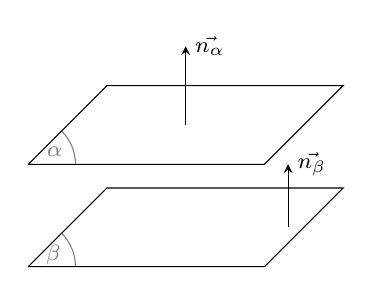
\begin{tikzpicture}[scale=1, font=\footnotesize,>=stealth]
	\path
	%	Vẽ mp
	(0,0) coordinate (A)
	(3,0) coordinate (B)
	(4,1) coordinate (C)
	(1,1) coordinate (D)
	(0,1.3) coordinate (E)
	(3,1.3) coordinate (F)
	(4,2.3) coordinate (G)
	(1,2.3) coordinate (H)
	;
	\draw 
	(A)--(B)--(C)--(D)--(A)
	(E)--(F)--(G)--(H)--(E)
	;
	\draw[->]
	(3.3,0.5)--(3.3,1.3)node[right]{$\vec{n_{\beta}}$};
	\draw[->]
	(2,1.8)--(2,2.8)node[right]{$\vec{n_{\alpha}}$};
	\begin{scope}
		\clip (B)--(A)--(D);
		\draw[opacity=0.5] (A) circle(0.6cm)node[black,shift={(25:3.5mm)}]{$\beta$};
	\end{scope}
	\begin{scope}
	\clip (F)--(E)--(H);
	\draw[opacity=0.5] (E) circle(0.6cm)node[black,shift={(25:3.7mm)}]{$\alpha$};
	\end{scope}
\end{tikzpicture}
\hspace{1cm}
\begin{tikzpicture}[scale=1, font=\footnotesize,>=stealth]
	\path
	%	Vẽ mp
	(0,0) coordinate (A)
	(3,0) coordinate (B)
	(4,1) coordinate (C)
	(1,1) coordinate (D)
	(2,0) coordinate (E)
	(3,1) coordinate (F)
	(3,3) coordinate (G)
	($(E)+(G)-(F)$)coordinate (H)
	(2,1) coordinate (i)
	(1,0.2) coordinate (M)
	(1.8,0.6) coordinate (N)
	;
	\draw 
	(A)--(B)--(C)--(F) (i)--(D)--(A)
	(E)--(F)--(G)--(H)--(E)
	;
	\draw[dashed]
	(F)--(i);
	\draw[->]
	(3.3,0.5)--(3.3,1.5)node[right]{$\vec{n_{\beta}}$};
	\draw[->]
	(2.6,2)--(3.7,2)node[above]{$\vec{n_{\alpha}}$};
	\draw[->](M)--(N);
	\begin{scope}
		\clip (B)--(A)--(D);
		\draw[opacity=0.5] (A) circle(0.6cm)node[black,shift={(25:3.5mm)}]{$\beta$};
	\end{scope}
	\begin{scope}
		\clip (E)--(H)--(G);
		\draw[opacity=0.5] (H) circle(0.3cm)node[black,shift={(-10:2mm)}]{$\alpha$};
	\end{scope}
\foreach \x/\g in {M/90,N/100}\draw[fill=black] (\x) circle (.03) +(\g:.17)node{\tiny$\x$};
\end{tikzpicture}
\hspace{1cm}
\begin{tikzpicture}[scale=1, font=\footnotesize,>=stealth]
	\path
	%	Vẽ mp
	(0,0) coordinate (A)
	(5.3,0) coordinate (B)
	(6.3,1) coordinate (C)
	(1,1) coordinate (D)
	(2,0) coordinate (E)
	(3,1) coordinate (F)
	(3,3) coordinate (G)
	($(E)+(G)-(F)$)coordinate (H)
	(4,1) coordinate (I)
	(5,0) coordinate (K)
	(5,2) coordinate (L)
	($(L)+(I)-(K)$)coordinate (M)
	(2,1) coordinate (i)
	(5,1) coordinate (j)
	;
	\draw 
	(A)--(B)--(C)--(j) (I)--(F) (i)--(D)--(A)
	(E)--(F)--(G)--(H)--(E)
	(I)--(K)--(L)--(M)--(I)
	;
	\draw[dashed]
	(F)--(i) (I)--(j);
	\draw[->]
	(1.4,0.5)--(1.4,2)node[left]{$\vec{n_{\beta}}$};
	\draw[->]
	(2.6,2)--(3.7,2)node[above]{$\vec{n_{\alpha_1}}$};
	\draw[->]
	(4.5,1.8)--(3.5,1.6)node[below]{$\vec{n_{\alpha_2}}$};
	\begin{scope}
		\clip (B)--(A)--(D);
		\draw[opacity=0.5] (A) circle(0.6cm)node[black,shift={(25:3.5mm)}]{$\beta$};
	\end{scope}
	\begin{scope}
		\clip (E)--(H)--(G);
		\draw[opacity=0.5] (H) circle(0.4cm)node[black,shift={(-10:2mm)}]{$\alpha_1$};
	\end{scope}
	\begin{scope}
		\clip (K)--(L)--(M);
		\draw[opacity=0.5] (L) circle(0.4cm)node[black,shift={(200:2mm)}]{$\alpha_2$};
	\end{scope}
\end{tikzpicture}
\end{dang}
\setcounter{ex}{0}
\setcounter{vd}{0}
\boxmini{BÀI TẬP TỰ LUẬN}

\begin{vd}
	Cho hai mặt phẳng $(P_1)\colon x - y - 2 z + 4 = 0$ và $(P_2)\colon x - y + z + 5 = 0$.	Chứng minh rằng $(P_1) \perp (P_2)$.
	\loigiai{
		Hai mặt phẳng $(P_1)$, $(P_2)$ có vectơ pháp tuyến lần lượt là $$\overrightarrow{n}_1 = (1; -1; -2), \overrightarrow{n}_2 = (1; -1; 1).$$
		Vì $\overrightarrow{n}_1 \cdot \overrightarrow{n}_2 = 1 \cdot 1 + (-1) \cdot (-1) + (-2) \cdot 1 = 0$ nên $\overrightarrow{n}_1 \perp \overrightarrow{n}_2$.\\
		Vậy $(P_1) \perp (P_2)$.
	}
\end{vd}

\dongcham{2}
\begin{vd}
	Trong không gian $Oxyz$, cho mặt phẳng $(\alpha)\colon 2x-3y+z+5=0$.
	\begin{listEX}[1]
		\item Chứng minh rằng mặt phẳng $\left(\alpha'\right)\colon-4 x+6 y-2 z+7=0$ song song với $(\alpha)$.
		\item Viết phương trình mặt phẳng $(\beta)$ đi qua điểm $M(1 ; -2 ; 3)$ và song song với $(\alpha)$.
	\end{listEX}
	\loigiai{
		\begin{listEX}[1]
			\item Xét $(\alpha)\colon 2x-3y+z+5=0$ và $\left(\alpha'\right)\colon -4x+6y-2z+7=0$.\\
			Ta có $\dfrac{2}{-4}=\dfrac{-3}{6}=\dfrac{1}{-2} \neq \dfrac{5}{7}$ nên $(\alpha) \parallel \left(\alpha'\right)$.
			\item Mặt phẳng $(\alpha)$ có véc-tơ pháp tuyến $\vec{n}=(2 ;-3 ; 1)$.\\
			Vì $(\beta) \parallel (\alpha)$ nên $(\beta)$ có véc-tơ pháp tuyến $\vec{n}=(2 ;-3 ; 1)$.\\
			Vậy mặt phẳng $(\beta)$ đi qua điểm $M(1 ;-2 ; 3)$ và có véc-tơ pháp tuyến $\vec{n}=(2 ;-3 ; 1)$ nên có phương trình là
			\allowdisplaybreaks
			\begin{eqnarray*}
				2(x-1)-3(y+2)+(z-3)=0 \qquad \text{hay } 2x-3y+z-11=0.
			\end{eqnarray*}
		\end{listEX}
		
	}
\end{vd}

\dongcham{5}

\begin{vd}
	Cho hai mặt phẳng $(P_1)\colon 2x - y - 3z + 1 = 0$ và $(P_2)\colon 6x - 3y - 9z + 1 = 0$.	
	\begin{enumEX}[a)]{1}
		\item Chứng minh rằng $(P_1) \parallel (P_2)$.
		\item Viết phương trình mặt phẳng $(P)$ cách đều $(P_1)$ và $(P_2)$.
	\end{enumEX}
	\loigiai{
		a) Hai mặt phẳng $(P_1)$, $(P_2)$ có vectơ pháp tuyến lần lượt là
		$$\overrightarrow{n}_1=(2 ;-1 ;-3), \overrightarrow{n}_2=(6 ;-3 ;-9).$$
		Vì $\overrightarrow{n}_2 = 3 \overrightarrow{n}_1$ và $D_1 = 1 \neq 3 \cdot 1 = 3 D_1$ nên $(P_1) \parallel (P_2)$.\\\\
		b) Ta có $(P_2): 6x-3y-9z+1=0\Leftrightarrow 2x-y-3z+\dfrac{1}{3}=0$.\\
		Phương trình mặt phẳng $(P)$ có dạng: $2x-y-3z+D=0$.\\
		Vì $(P)$ cách đều $(P_1)$ và $(P_2)$ nên $D=\dfrac{1+\frac{1}{3}}{2}=\dfrac{2}{3}$.\\
		Vậy phương trình mặt phẳng $(P)$ là $2x-y-3z+\dfrac{2}{3}=0$.
	}
\end{vd}
\dongcham{6}
\begin{vd}
	Cho  hai mặt phẳng $(Q) \colon x+y+3z=0$, $(R) \colon  2x-y+z=0$.
	\begin{enumEX}[a)]{1}
		\item Xét vị trí tương đối của $(Q)$ và $(R)$;
		\item Viết trình của mặt phẳng $(P)$ đi qua điểm $B(2;1;-3)$, đồng thời vuông góc với $(Q)$ và $(R)$.
	\end{enumEX}
	\loigiai{a) Ta có $\vec{n}_Q=(1;1;3), \vec{n}_R=(2;-1;1)$. Vì $\dfrac{1}{2}\ne\dfrac{1}{-1}$ nên $\vec{n}_Q$ không cùng phương với $\vec{n}_R$.\\
		Vậy $(Q)$ và $(R)$ cắt nhau.\\\\
		b) Véc tơ pháp tuyến $(P)$ là $\vec{n}_{P}= \left[ \vec{n}_Q,\vec{n}_R \right]= (4;5;-3)$.\\
		Phương trình mặt phẳng $(P)$ là $4(x-2)+5(y-1)-3(z+3)=0 \Leftrightarrow 4x+5y-3z-22=0$.
	}
\end{vd}
\dongcham{7}
\begin{vd}%[Đề tập huấn, Sở GD - ĐT tỉnh Quảng Bình, 2019]%[Nguyễn Tiến, dự án 12EX5]%[2H3K2-3]%
	Trong không gian với hệ tọa độ $Oxyz$, cho hai điểm $A(-2;4;-1)$, $B(1;1;3)$ và mặt phẳng $(P)$ có phương trình $x-3y+2z-5=0$. Viết phương trình mặt phẳng $(Q)$ đi qua hai điểm $A$, $B$ đồng thời vuông góc với mặt phẳng $(P)$.
	\loigiai{
		$\left.\begin{array}{l} \overrightarrow{AB}=(3;-3;4)\\ \overrightarrow{n}_{(P)}=(1;-3;2)\end{array}\right\}\Rightarrow\left[\overrightarrow{AB},\overrightarrow{n}_{(P)}\right]=(6;-2;-6)=2(3;-1;-3)$.\\
		Mặt phẳng $(Q)$ đi qua điểm $A$ và có vec-tơ pháp tuyến $\overrightarrow{n}_{(Q)}=(3;-1;-3)$ có phương trình
		\begin{eqnarray*}
			& & 3(x+2)-(y-4)-3(z+1)=0\\
			&\Leftrightarrow & 3x-y-3z+7=0.
		\end{eqnarray*}
	}
\end{vd}
\dongcham{10}

\boxmini{BÀI TẬP TRẮC NGHIỆM}

\begin{ex}%[2H3B2-7]
	Cho mặt phẳng $(P)\colon -x+y+3z+1=0$. Mặt phẳng song song với mặt phẳng $(P)$ có phương trình nào sau đây?
	\choice
	{\True $2x-2y-6z+7=0$}
	{$-2x+2y+3z+5=0$}
	{$x-y+3z-3=0$}
	{$-x-y+3z+1=0$}
	\loigiai{
		Véc-tơ pháp tuyến của mặt phẳng $ (P) $ là $ \overrightarrow{n}=(-1;1;3)$ cùng phương với véc-tơ $\overrightarrow{n}=(2;-2;-6) $. Vì $ \dfrac{2}{-1}\neq \dfrac{7}{1} $ nên phương trình mặt phẳng song song với $ (P) $ là $2x-2y-6z+7=0$.
	}
\end{ex}
\cham{2}

\begin{ex}
	Trong không gian với hệ tọa độ $O x y z$ cho ba mặt phẳng $(P)$, $(Q)$, $(R)$ tương ứng có phương trình là $2 x+6 y-4 z+8=0$; $5 x+15 y-10 z+20=0$ và $6 x+18 y-12 z-24=0$. Chọn mệnh đề đúng trong bốn mệnh đề sau
	\choice
	{$(P) \parallel (Q)$}
	{$(P)$ cắt $(Q)$}
	{$(Q)$ cắt $(R)$}
	{\True $(R) \parallel (P)$}
	\loigiai{
		Thu gọn phương trình tổng quát của $ 3 $ mặt phẳng đã cho, ta được
		\begin{align*}
			&(P): x+3 y-2 z+4=0 \\
			&(Q): x+3 y-2 z+4=0 \\
			&(R): x+3 y-2 z-4=0
		\end{align*}
		Dễ thấy $ (P) \parallel (R) $.
	}
\end{ex}
\cham{2}
\begin{ex}%[2H3B2-7]
	Cho hai mặt phẳng $(P) \colon 2x+4y+3z-5=0$ và $(Q) \colon mx-ny-6z+2-0$. Giá trị của $m,n$ sao cho $(P) \parallel (Q)$ là
	\choice
	{$m=4;n=-8$}
	{$m=n=4$}
	{\True $m=-4;n=8$}
	{$m=n=-4$}
	\loigiai{
		$(P)$ có véc-tơ chỉ phương $\overrightarrow{u}_{(P)}=(2;4;3)$, $(Q)$ có véc-tơ chỉ phương $\overrightarrow{u}_{(Q)}=(m;-n;-6)$.\\ Để hai mặt phẳng trên song song thì $\overrightarrow{u}_{(Q)}=k\overrightarrow{u}_{(P)}\,(k \neq 0) \Leftrightarrow \heva{&m=2k\\&-n=4k\\&-6=3k} \Rightarrow \heva{&k=-2\\&m=-4\\&n=8.}$
	}
	
\end{ex}
\cham{3}

\begin{ex}
	Cho hai mặt phẳng $(P)\colon x+my+(m-1)z+1=0$ và $(Q)\colon x+y+2z=0$. Tập hợp tất cả các giá trị $m$ để hai mặt phẳng này \textbf{không} song song là
	\choice
	{$(0;+\infty)$}
	{$\mathbb{R}\setminus\{-1;1;2\}$}
	{$(-\infty;3)$}
	{\True $\mathbb{R}$}
	\loigiai{
		Ta có $A(0;0;0)\in (Q)$.\\
		$(P)\parallel (Q)\Leftrightarrow \heva{&\dfrac{1}{1}=\dfrac{m}{1}=\dfrac{m-1}{2}\\&A(0;0;0)\notin (P)}$. Hệ này vô nghiệm. Do đó $(P)$ không song song với $(Q)$, với mọi giá trị của $m$. 
	} 
\end{ex}
\cham{4}

\begin{ex}
	Cho mặt phẳng $(\alpha)\colon x+y+z-1=0$. Trong các mặt phẳng sau, tìm mặt phẳng vuông góc với mặt phẳng $(\alpha)$.
	\choice
	{$2x-y+z+1=0$}
	{\True $2x-y-z+1=0$}
	{$2x+2y+2z-1=0$}
	{$x-y-z+1=0$}
	\loigiai{
		Mặt phẳng $(\alpha)$ có $\overrightarrow{n}_{(\alpha)}=(1;1;1)$.\\
		Mặt phẳng $2x-y-z+1=0$ có vec-tơ pháp tuyến $\overrightarrow{n}_1=(2;-1;-1)\Rightarrow\overrightarrow{n}_{(\alpha)}\cdot\overrightarrow{n}_1=0$ nên mặt phẳng $(\alpha)$ vuông góc với mặt phẳng $2x-y-z+1=0$.
	}
\end{ex}
\cham{2}
\begin{ex}%[2H3B2-7]
	Cho mặt phẳng $(P)\colon 2x-y+2z-3=0$ và $(Q) \colon x+my+z-1=0$. Tìm tham số $m$ để hai mặt phẳng $P$ và $Q$ vuông góc với nhau.
	\choice
	{$m=-4$}
	{$m=- \dfrac{1}{2}$}
	{$m=\dfrac{1}{2}$}
	{\True $m=4$}
	\loigiai
	{ Mặt phẳng $(P)$ và $(Q)$ có véc-tơ pháp tuyến lần lượt là $\overrightarrow{n}_1=(2;-1;2)$ và $\overrightarrow{n}_2=(1;m;1)$. \\
		Do đó $(P) \perp (Q) \Leftrightarrow \overrightarrow{n}_1 \cdot \overrightarrow{n}_2=0 \Leftrightarrow 2-m+2=0 \Leftrightarrow m=4$.
		
	}
\end{ex}
\cham{2}

\begin{ex}
	Cho hai mặt phẳng $(P)\colon x+2y-z-1=0$, $(Q)\colon 3x-(m+2)y+(2m-1)z+3=0$. Tìm $m$ để hai mặt phẳng $(P)$ và $(Q)$ vuông góc với nhau.
	\choice
	{\True $m=0$}
	{$m=2$}
	{$m=-2$}
	{$m=-1$}
	\loigiai{
		Véc-tơ pháp tuyến của $(P)$, $(Q)$ lần lượt là $\overrightarrow{n}_P=(1;2;-1)$ và $\overrightarrow{n}_Q=(3;-m-2;2m-1)$.\\
		$(P)\perp (Q)\Leftrightarrow \overrightarrow{n}_P\cdot\overrightarrow{n}_Q=0\Leftrightarrow 3-2(m+2)-2m+1=0\Leftrightarrow m=0$.
	}
\end{ex}
\cham{2}
\begin{ex}%[2H3B2-3]%
	Mặt phẳng đi qua $A(1;3;-2)$ và song song với mặt phẳng $(P) \colon 2x-y+3z+4=0$ có phương trình là
	\choice
	{\True $2x-y+3z+7=0$}
	{$2x-y+3z-7=0$}
	{$2x+y-3z+7=0$}
	{$2x+y+3z+7=0$}
	\loigiai{
		Ta có $\vec{n}=\vec{n_{(P)}}=(2;-1;3)$. Khi đó phương trình mặt phẳng qua $A(1;3;-2)$ và song song $(P)$ là
		$$2(x-1)-1(y-3)+3(z+2)=0\Leftrightarrow 2x-y+3z+7=0.$$
	}
\end{ex}
\cham{2}

\begin{ex}%[KSCL giữa HK2 Cụm trường THPT TP Nam Định]%[Nguyễn Tiến, 12EX7]%[2H3B2-3]%
	Cho điểm $A(2;-1;-3)$ và mặt phẳng $(P)\colon 3x-2y+4z-5=0$. Mặt phẳng $(Q)$ đi qua $A$ và song song với mặt phẳng $(P)$ có phương trình là
	\choice
	{\True $(Q)\colon 3x-2y+4z+4=0$}
	{$(Q)\colon 3x+2y+4z+8=0$}
	{$(Q)\colon 3x-2y+4z+5=0$}
	{$(Q)\colon 3x-2y+4z-4=0$}
	\loigiai{
		Do mặt phẳng $(Q)$ song song với mặt phẳng $(P)$ nên có vectơ pháp tuyến là $\overrightarrow{n}=(3;-2;4)$.\\
		Phương trình mặt phẳng $(Q)\colon 3(x-2)-2(y+1)+4(z+3)=0 \Leftrightarrow 3x-2y+4z+4=0$.
	}
\end{ex}
\cham{2}
\begin{ex}
	Cho mặt phẳng $(P)$ đi qua các điểm $A(-2; 0; 0)$, $B(0; 3; 0)$, $C(0; 0; -3)$. Mặt phẳng $(P)$ vuông góc với mặt phẳng nào trong các mặt phẳng sau?
	\choice
	{\True $2x+2y-z-1=0$}
	{$x+y+z+1=0$}
	{$3x-2y+2z+6=0$}
	{$x-2y-z-3=0$}
	\loigiai{
		Mặt phẳng $(P)\colon \dfrac{x}{-2}+\dfrac{y}{3}+\dfrac{z}{-3}=1$ hay $(P)\colon 3x-2y+2z+6=0$ có véc-tơ pháp tuyến $\vec{n}=(3;-2;2)$.\\
		Ta có $3\cdot 2 -2\cdot 2-2\cdot 1=0$ nên $(P)$ vuông góc với mặt phẳng $2x+2y-z-1=0$.
	}
\end{ex}
\cham{2}
\begin{ex}
	Mặt phẳng qua $A(1;2;-1)$ và vuông góc với các mặt phẳng $(P) \colon 2x-y+3z-2=0$; $(Q) \colon x+y+z-1=0$ có phương trình là
	\choice
	{$x-y+z+2=0$}
	{$4x-y+z-1=0$}
	{$x+y+2z-1=0$}
	{\True $4x-y-3z-5=0$}
	\loigiai{
		Véc-tơ pháp tuyến của mặt phẳng $(P)$ và $(Q)$ lần lượt là $\overrightarrow{n_1}=(2;-1;3)$ và $\overrightarrow{n_2}=(1;1;1)$.
		\\
		Ta có $\left[\overrightarrow{n_1};\overrightarrow{n_2}\right]=(-4;1;3)$.
		Mặt phẳng cần tìm qua $A(1;2;-1)$ và có véc-tơ pháp tuyến là $\overrightarrow{n}=(-4;1;3)$ nên có phương trình là
		$$-4 \cdot (x-1)+1 \cdot (y-2)+3 \cdot (z+1)=0\Leftrightarrow4x-y-3z-5=0.$$}
\end{ex}
\cham{2}
\begin{ex}
	Cho hai mặt phẳng $(P)$, $(Q)$ lần lượt có phương trình là $x+y-z=0$, $x-2y+3z=4$ và cho điểm $M(1;-2;5)$. Tìm phương trình mặt phẳng $(\alpha)$ đi qua điểm $M$ và đồng thời vuông góc với hai mặt phẳng $(P)$, $(Q)$.
	\choice
	{$5x+2y-z+14=0$}
	{\True $x-4y-3z+6=0$}
	{$x-4y-3z-6=0$}
	{$5x+2y-z+4=0$}
	\loigiai{
		Ta có $\vec{n}_{(P)} = (1;1;-1)$ và
		$\vec{n}_{(Q)} = (1;-2;3).$\\
		Suy ra $\left[\vec{n}_{(P)},\vec{n}_{(Q)}\right]= (1;-4;-3).$\\
		Do $(\alpha)$ vuông góc với $(P)$ và $(Q)$ nên $\heva{&\vec{n}_{(\alpha)} \perp \vec{n}_{(P)}\\&\vec{n}_{(\alpha)} \perp \vec{n}_{(Q)}}$. \\
		Chọn $\vec{n}_{(\alpha)} = \left[\vec{n}_{(P)},\vec{n}_{(Q)}\right]=(1;-4;-3)$. Hơn nữa, $(\alpha)$ đi qua $M(1;-2;5)$ nên có phương trình là $$(x-1)-4(y+2)-3(z-5)=0\Leftrightarrow x-4y-3z+6=0.$$
	}
\end{ex}
\cham{2}
\begin{ex}%[Thi thử, THPT chuyên Quang Trung, 2020]%[Phạm Doãn Lê Bình, 12EX2-2020]%[2H3B2-3]%
	Cho điểm $A(-4;1;1)$ và mặt phẳng $(P)\colon x-2y-z+4=0$. Mặt phẳng $(Q)$ đi qua điểm $A$ và song song với mặt phẳng $(P)$ có phương trình là
	\choice
	{\True $(Q)\colon x-2y-z+7=0$}
	{$(Q)\colon x-2y-z-7=0$}
	{$(Q)\colon x-2y+z+5=0$}
	{$(Q)\colon x-2y+z-5=0$}
	\loigiai{
		Do $(Q)\parallel (P)$ nên phương trình của $(Q)$ có dạng $x-2y-z+c=0$ ($c\ne 4$).\\
		Do $A \in (Q)$ nên $-4-2\cdot 1 - 1 + c = 0 \Leftrightarrow c = 7$ (thỏa).\\
		Vậy $(Q)\colon x-2y-z+7=0$.
	}
\end{ex}
\cham{2}
\begin{ex}%[Thi thử L1, THPT Chuyên ĐH Vinh, Nghệ An, 2019]%[Nguyễn Đắc Giáp, dự án 12EX6]%[2H3B2-3]%
	Cho hai mặt phẳng $(P)\colon x-3y+2z-1=0$, $(Q)\colon x-z+2=0$. Mặt phẳng $\left(\alpha\right)$ vuông góc với hai mặt phẳng $(P),(Q)$ đồng thời cắt trục $Ox$ tại điểm có hoành độ bằng $3$. Phương trình của $\left(\alpha\right)$ là
	\choice
	{$-2x+z+6=0$}
	{$-2x+z-6=0$}
	{\True $x+y+z-3=0$}
	{$x+y+z+3=0$}
	\loigiai{
		Mặt phẳng $(P)$ có một véc-tơ pháp tuyến là $\overrightarrow{n}_P=(1;-3;2)$.\\
		Mặt phẳng $(Q)$ có một véc-tơ pháp tuyến là $\overrightarrow{n}_Q=(1;0;-1)$.\\
		Vì mặt phẳng $(\alpha)$ vuông góc với hai mặt phẳng $(P)$ và $(Q)$ nên $(\alpha)$ có một véc-tơ pháp tuyến là	 $\overrightarrow{n}_{\alpha}=\left[\overrightarrow{n}_P,\overrightarrow{n}_Q\right]=3(1;1;1)$.\\
		Mà mặt phẳng $(\alpha)$ đi qua $A(3;0;0)$, nên suy ra phương trình là $\left(\alpha\right)\colon x+y+z-3=0$.
	}
\end{ex}
\cham{2}
\begin{ex}%[2H3K2-3]%
	Cho $A\left( 1;-1;2 \right);\ B\left( 2;1;1 \right)$ và mặt phẳng $\left( P \right):x+y+z+1=0$. Mặt phẳng $\left( Q \right)$ chứa $A,\ B$ và vuông góc với mặt phẳng $\left( P \right)$. Mặt phẳng $\left( Q \right)$ có phương trình là
	\choice
	{$3x-2y-z+3=0$}
	{\True $3x-2y-z-3=0$}
	{$-x+y=0$}
	{$x+y+z-2=0$}
	\loigiai
	{
		Ta có $\vec{A B}=(1 ; 2 ;-1)$ và véc-tơ pháp tuyến của $(P)$ là $\vec{n}_{P}=(1 ; 1 ; 1)$. Gọi véc-tơ pháp tuyến của $(Q)$ là $\vec{n}_{Q}$.\\
		Vì $(Q)$ chứa $A,B$ nên $\vec{n_{Q}} \perp \vec{A B}$, mặt khác $(Q) \perp(P)$ nên $\vec{n_{Q}} \perp \vec{n_{P}}$. \\
		Từ đó suy ra $\vec{n_{Q}}=\left[\vec{A B}, \vec{n_{P}}\right]=(3 ;-2 ;-1)$.\\
		$(Q)$ đi qua $A(1;-1;2)$ và có véc-tơ pháp tuyến $\vec{n_{Q}}=(3 ;-2 ;-1)$ nên $(Q)$ có phương trình là
		$$(Q):3(x-1)-2(y+1)-(z-2)=0 \Leftrightarrow 3 x-2 y-z-3=0.$$
	}
\end{ex}
\cham{2}
\begin{ex}%[2H3K2-3]%[Đề thi thử L2, THPT Nguyễn Quang Diêu, 2018]%[Đỗ Đường Hiếu, 12EX-9]%
	Cho hai điểm $A(2;4;1)$, $B(-1;1;3)$ và mặt phẳng $(P)\colon x-3y+2z-5=0$. Một mặt phẳng $(Q)$ đi qua hai điểm $A$, $B$ và vuông góc với mặt phẳng $(P)$ có dạng là $ax+by+cz-11=0$. Tính $a+b+c$.
	\choice
	{$a+b+c=-7$}
	{$a+b+c=10$}
	{\True $a+b+c=5$}
	{$a+b+c=3$}
	\loigiai{
		Ta có $\overrightarrow{AB}=\left(-3;-3;2\right)$ và véc-tơ pháp tuyến của mặt phẳng $(P)$ là $\overrightarrow{n}_P=\left(1;-3;2\right)$.\\
		Mặt phẳng $(Q)$ đi qua hai điểm $A$, $B$ và vuông góc với mặt phẳng $(P)$ có một véc-tơ chỉ phương là
		$$\overrightarrow{n}_Q=\left[\overrightarrow{AB}, \overrightarrow{n}_P\right]=\left(0;8;12\right) =4\left(0;2;3\right).$$
		Phương trình mặt phẳng $(Q)$ là
		$$0\cdot (x-2)+2\cdot (y-4)+3\cdot (z-1)=0.$$
		Hay $(Q)\colon 2y+3z-11=0$.
		Từ đó suy ra $a=0$, $b=2$, $c=3$. Do đó $a+b+c=0+2+3=5$.
	}
\end{ex}
\cham{2}
\begin{dang}{Khoảng cách}
	\begin{itemize}
		\item [\iconCV] \indamm{Khoảng cách từ một điểm đến mặt phẳng:} Cho điểm $M(x_0;y_0;z_0)$ và mặt phẳng $(P) \colon ax+by+cz+d=0$. Khi đó
	$\mathrm{d}\left(M,(P) \right)=\dfrac{\bigg|ax_0+by_0+cz_0+d\bigg|}{\sqrt{a^2+b^2+c^2}}$
		\item [\iconCV] \indamm{Khoảng cách giữa hai mặt phẳng song song:} 	Cho $(P) \colon ax + by + cz + d_1=0$ và $(Q) \colon ax + by + cz + d_2=0$ song song nhau. 
		Khi đó
		$\mathrm{d}\left((P),(Q) \right)=\dfrac{\bigg|d_1-d_2\bigg|}{\sqrt{a^2+b^2+c^2}}$
	\end{itemize}
\end{dang}
\setcounter{ex}{0}
\setcounter{vd}{0}
\boxmini{BÀI TẬP TỰ LUẬN}
\begin{vd}%[2H5H1-5] %[Dang]
	Tính khoảng cách từ điểm $A(1;2;3)$ đến các mặt phẳng sau
	\begin{enumEX}[a)]{2}
		\item $\left(P\right) \colon 3x + 4z + 10 = 0$;
		\item $\left(Q\right) \colon 2x + 2y + z - 3 = 0$;
		\item $\left(R\right) \colon 2x - 10 = 0$;
		\item $\left(S\right) \colon z=4$;
	\end{enumEX}
	
	\loigiai{
		\begin{listEX}
			\item $\mathrm{d}\left( A;\left( P \right) \right) = \dfrac{\left| {3 \cdot 1 + 0 \cdot 2 + 4 \cdot 3 + 10} \right|}{\sqrt {3^2 + 4^2}} = 5$.
			\item $\mathrm{d}\left( A;\left( Q \right) \right) = \dfrac{\left| {2 \cdot 1 + 2 \cdot 2 + 1 \cdot 3 - 3} \right|}{\sqrt {2^2 + 2^2 + 1^2} } = 2$.
			\item $\mathrm{d}\left(A;\left( R \right) \right) = \dfrac{\left| {2 \cdot 1 - 10} \right|}{\sqrt {2^2} } = 4$.
			\item $\mathrm{d}\left( A;\left( S \right) \right) = \dfrac{\left| {z_A-4} \right|}{\sqrt {0^2 + 0^2 + 1^2} } = 1$.
		\end{listEX}
	}
\end{vd}
\dongcham{3}
\begin{vd}%[2H5N1-4]%[2H5H1-5]%[Dự án tex hóa sách bài tập Toán 12 CTST]%[Lê Thị Thúy Hằng]
	Cho hai mặt phẳng $(P) \colon 2x+y+2z+12=0$, $(Q) \colon 4x+2y+4z-6=0$.
	\begin{enumerate}
		\item Chứng minh $(P) \parallel (Q)$.
		\item Tính khoảng cách giữa hai mặt phẳng $(P)$ và $(Q)$.
	\end{enumerate}
	\loigiai{
		\begin{enumerate}
			\item Xét hai mặt phẳng $(P) \colon 2x+y+2z+12=0$ và $(Q) \colon 4x+2y+4z-6=0$, ta có
			$\dfrac{4}{2} = \dfrac{2}{1} = \dfrac{4}{2} \ne \dfrac{-6}{12}$, suy ra $(P) \parallel (Q)$.
			\item Trên mặt phẳng $(Q)$, lấy điểm $M(0;1;1)$.\\
			Ta có
			$$ \mathrm{d}((P),(Q)) = \mathrm{d} (M, (P)) = \dfrac{\left| 2 \cdot 0 + 1 \cdot 1 + 2 \cdot 1 + 12 \right|}{\sqrt{2^2+1^2+2^2}}=\dfrac{15}{3}=5.$$
		\end{enumerate}
	}
\end{vd}
\dongcham{7}
\begin{vd}
	\immini{
		Một kĩ sư xây dựng thiết kế khung một ngôi nhà trong không gian $Oxyz$ như hình bên nhờ một phần mềm đồ họa máy tính.
		\begin{enumerate}
			\item Viết phương trình mặt phẳng mái nhà $(DEMN)$.
			\item Tính khoảng cách từ điểm $B$ đến mái nhà $(DEMN)$.
		\end{enumerate}
	}
	{
		\begin{tikzpicture}[scale=.7, font=\footnotesize, line join=round, line cap=round, >=stealth]
			\path 
			(0:0) coordinate (O)
			(-135:2) coordinate (A)
			(0:4) coordinate (C)
			($(A)+(-135:1)$) coordinate (x)
			($(A)+(45:2)$) coordinate (O)
			($(A)+(C)-(O)$) coordinate (B)
			($(O)+(90:4)$) coordinate (D)
			($(D)+(90:1.2)$) coordinate (z)
			($(C)+(0:1)$) coordinate (y)
			($(A)+(90:4)$) coordinate (E)
			($(B)+(90:4)$) coordinate (F)
			($(C)+(90:4)$) coordinate (H)
			($(D)+(20:2)$) coordinate (N)
			($(E)+(20:2)$) coordinate (M)
			($(O)+(-50:4.5)$) coordinate (h)
			;
			\draw[dashed] (A)--(O)--(C) (O)--(D)--(H);
			\draw[->] (A)--(x) node[below]{$x$};
			\draw[->](C)--(y) node[above]{$y$};
			\draw[->](D)--(z) node[right]{$z$};
			\draw 	(B)--(F)--(E)--(A)--cycle
			(D)--(E)--(M)--(N)--cycle
			(B)--(C)--(H)--(F)--(M) (N)--(H) 
			;
			\draw (A) node[left]{$A(6;0;0)$}
			(O) node[below right]{$O(0;0;0)$}
			(C) node[below right]{$C(0;4;0)$}
			(D) node[left]{$D(0;0;4)$}
			(M) node[right]{$M(6;2;6)$}
			(N) node[above right]{$N(0;2;6)$}
			(E) node[left]{$E(6;0;4)$}
			(B) node[right]{$B$}
			(H) node[right]{$H$}
			;
			%pic[draw,angle radius=2mm]{right angle=C--O--O'}
			%pic[draw,angle radius=2mm]{right angle=A--O--C}
			%pic[draw,angle radius=2mm]{right angle=O'--O--A}
			%;
			%\foreach \x/\g in {A/170,B/-15,C/-30,O/180,E/170,F/-15,H/0,D/180}
			%\draw[fill=black] 	(\x) circle (.5pt)
			%($(\g:.5)+(\x)$) node {$\x$};	
		\end{tikzpicture}
	}
	\loigiai{
		\begin{enumerate}
			\item Mặt phẳng $(DEMN)$ có cặp véc-tơ chỉ phương là $\overrightarrow{DE} =(6;0;0)$, $\overrightarrow{DN} = (0;2;2)$. Ta có $\left[ \overrightarrow{DE}, \overrightarrow{DN} \right] =(0;-12;12)$, suy ra $(DEMN)$ có véc-tơ pháp tuyến là $$\overrightarrow{n} = -\dfrac{1}{12} \left[ \overrightarrow{DE}, \overrightarrow{DN} \right] = (0;1;-1).$$
			Phương trình của mặt phẳng $(DEMN)$ là $y-z+4=0$.
			\item $B(6;4;0)$, suy ra $\mathrm{d} (B,(DEMN)) = \dfrac{\left| 4+4 \right|}{\sqrt{0^2+1^2+(-1)^2}} = \dfrac{8}{\sqrt{2}} = 4\sqrt{2}$.
		\end{enumerate}
	}
\end{vd}
\dongcham{7}
\begin{vd}
	\immini{Cho hình hộp chữ nhật $ABCD.A'B'C'D'$ có $DA=2$, $DC=3$, $DD'=2$. 
		\begin{enumEX}[a)]{1}
			\item Tính khoảng cách từ đỉnh $B'$ đến mặt phẳng $(BA'C')$.
			\item  Gọi $G$ là trọng tâm tam giác $ABC$, $M$ là điểm trên $AD'$ thỏa $\vec{AM}=\dfrac{1}{3}\vec{AD'}$. Tính độ dài đoạn $GM$.
		\end{enumEX}
	}{
\begin{tikzpicture}[scale=0.7, font=\footnotesize, line join=round, line cap=round, >=stealth]
	\path 
	(0,0) coordinate (D)
	($(D)+(-135:2)$) coordinate (A)
	($(A)+(-135:1)$) coordinate (x)
	(0:4.5) coordinate (C)
	($(C)+(0:1)$) coordinate (y)
	($(A)+(C)-(D)$) coordinate (B)
	($(D)+(90:3)$) coordinate (D')
	($(D')+(90:1)$) coordinate (z)
	($(A)+(90:3)$) coordinate (A')
	($(B)+(90:3)$) coordinate (B')
	($(C)+(90:3)$) coordinate (C')
	;
	\draw[dashed] (A)--(D)--(C)--cycle (D)--(D');
	\draw (A')--(A)--(B)--(B')--(A')--(B')--(C')--(D') (B)--(C)--(C')--(B') (D')--(A')--(C')--(B);
	\draw[->] (A')--(B);
	\foreach \x/\g in {A/170,B/-15,C/-60,D/180,D'/180,A'/180,B'/90,C'/12}\draw	(\x)($(\g:.35)+(\x)$) node {$\x$};	
\end{tikzpicture}}
	\loigiai{
		\begin{center}
			\begin{tikzpicture}[scale=1, font=\footnotesize, line join=round, line cap=round, >=stealth]
				\path 
				(0,0) coordinate (D)
				($(D)+(-135:2)$) coordinate (A)
				($(A)+(-135:1)$) coordinate (x)
				(0:4.5) coordinate (C)
				($(C)+(0:1)$) coordinate (y)
				($(A)+(C)-(D)$) coordinate (B)
				($(D)+(90:3)$) coordinate (D')
				($(D')+(90:1)$) coordinate (z)
				($(A)+(90:3)$) coordinate (A')
				($(B)+(90:3)$) coordinate (B')
				($(C)+(90:3)$) coordinate (C')
				;
				\draw[dashed] (A)--(D)--(C)--cycle (D)--(D');
				\draw (A')--(A)--(B)--(B')--(A')--(B')--(C')--(D') (B)--(C)--(C')--(B') (D')--(A')--(C')--(B);
				\draw[->] (A')--(B);
				\draw[->] (A)--(x) node[below]{$x$};
				\draw[->] (C)--(y) node[below]{$y$};
				\draw[->] (D')--(z) node[left]{$z$};
				\foreach \x/\g in {A/170,B/-15,C/-60,D/180,D'/180,A'/180,B'/90,C'/12}
				\draw	(\x)
				($(\g:.2)+(\x)$) node {$\x$};	
			\end{tikzpicture}
		\end{center}
		Chọn hệ tọa độ $Oxyz$ sao cho gốc tọa độ $O$ trùng với điểm $D$.\\
		Khi đó, tọa độ các đỉnh của hình hộp chữ nhật $ABCD.A'B'C'D'$ là 
		$D(0,0,0)$, $A(2,0,0)$, $C(0,3,0)$, $B(2,3,0)$, $D'(0,0,2)$, $A'(2,0,2)$, $B'(2,3,2)$, $C'(0,3,2)$.\\
		a) Mặt phẳng $(BA'C')$ có cặp véc-tơ chỉ phương là
		$\overrightarrow{BA'}=(0;-3;2)$, $\overrightarrow{BC'}=(-2;0;2)$. \\
		Ta có $\left[ \overrightarrow{BA'}, \overrightarrow{BC'} \right] =(-6;-4;-6)$, suy ra $(BA'C')$ có véc-tơ pháp tuyến là 
		$$\overrightarrow{n} = -\dfrac{1}{2} \left[ \overrightarrow{BA'}, \overrightarrow{BC'} \right] = (3;2;3).$$\\
		Phương trình của $(BA'C')$ là
		$$3(x-2)+2(y-3)+3z=0 \text{ hay } 3x+2y+3z-12=0.$$
		Khoảng cách từ đỉnh $B'$ đến mặt phẳng $(BA'C')$ là
		$$\mathrm{d} (B', (BA'C')) = \dfrac{\left| 3 \cdot 2 + 2 \cdot 3 + 3 \cdot 2 - 12 \right|}{\sqrt{3^2+2^2+3^2}}=\dfrac{6}{\sqrt{22}}=\dfrac{3 \sqrt{22}}{11}.$$
		
		b) Ta có $\vec{AD'}=(-2;0;2)$. Gọi $M(x;y;z)$. Khi đó: $\vec{AM}=(x-2;y;z)$.\\
		Vì $\vec{AM}=\dfrac{1}{3}\vec{AD'}$ nên $\heva{&x-2=\dfrac{1}{3}\cdot(-2)\\&y=0\\&z=\dfrac{1}{3}\cdot 2}\Leftrightarrow\heva{&x=\dfrac{4}{3}\\&y=0\\&z=\dfrac{2}{3}}\Rightarrow M\left(\dfrac{4}{3};0;\dfrac{2}{3}\right)$.\\
		Lại có $G$ là trọng tâm tam giác $ABC$ nên $G\left(\dfrac{4}{3};2;0\right)$.\\
		Do đó: $\vec{GM}=\left(0;-2;\dfrac{2}{3}\right)$. Vậy $GM=\sqrt{0+4+\dfrac{4}{9}}=\dfrac{2\sqrt{10}}{3}$.
	} 
\end{vd}
\dongcham{10}
\begin{vd}
	\immini{Cho hình chóp $S. ABCD$ có đáy $ABCD$ là hình vuông cạnh $a$, $SD=\dfrac{3a}{2}$, hình chiếu vuông góc của $S$ lên mặt phẳng $(ABCD)$ là trung điểm của cạnh $AB$. 
	\begin{enumEX}[a)]{1}
		\item Tính thể tích khối chóp $S.ABCD$ theo $a$.
		\item Tính khoảng cách $d$ từ $A$ đến mặt phẳng $(SBD)$. 
	\end{enumEX}
}{
\begin{tikzpicture}[line cap=round,line join=round,>=stealth,x=1.0cm,y=1.0cm,scale=.6]
	\path 
	(2,1) coordinate (A)
	(0,0) coordinate (B)
	(7,1) coordinate (D)
	($(D)+(B)-(A)$)coordinate (C)
	($(A)!0.5!(C)$) coordinate (O)
	($(A)!0.5!(B)$) coordinate (M)
	($(M)+(0,4)$) coordinate (S) 
	;
	\foreach \x/\g in{A/35,B/-90,C/-90,D/0,O/-90,S/90}
	\fill[black](\x) circle (1pt)($(\x)+(\g:4mm)$) node{\small $\x$};
	\draw (S)--(B) (S)--(C) (S)--(D) (B)--(C) (C)--(D); 
	\draw [dashed, thin] (S)--(A) (A)--(B) (A)--(D) (S)--(O) (A)--(C) (B)--(D) (S)--(M); 
\end{tikzpicture} }
	\loigiai{Gọi $H$ là trung điểm $AB$.\\
		a) Ta có: $HD=\sqrt{AH^2+AD^2}=\sqrt{\dfrac{a^2}{4}+a^2}=a\dfrac{\sqrt{5}}{2}$.\\
		Suy ra: $SH=\sqrt{SD^2-HD^2}=\sqrt{\dfrac{9a^2}{4}-\dfrac{5a^2}{4}}=a$.\\
		Vậy $V_{S.ABCD}=\dfrac{1}{3}\cdot SH\cdot S_{ABCD}=\dfrac{1}{3}\cdot a\cdot a^2=\dfrac{a^3}{3}$.\\\\
		b) Chọn hệ tọa độ $Oxyz$ sao cho gốc tọa độ $O$ trùng với điểm $H$.\\
		Khi đó, tọa độ các điểm là $H(0;0;0), A\left(-\dfrac{a}{2}; 0;0\right), B\left(\dfrac{a}{2};0;0\right), D\left(-\dfrac{a}{2};a;0\right), S(0;0;a)$.\\
		Mặt phẳng $(SBD)$ có cặp véc tơ chỉ phương là $\vec{BS}=\left(-\dfrac{a}{2};0;a\right), \vec{BD}=(-a;a;0)$.\\
		Ta có $\left[\vec{BS},\vec{BD}\right]=\left(-a^2;-a^2;-\dfrac{a^2}{2}\right)$, suy ra $(SBD)$ có véc tơ pháp tuyến là
		$$\vec{n}=-a^2\left[\vec{BS}, \vec{BD}\right]=\left(1;1;\dfrac{1}{2}\right).$$
		Phương trình của $(SBD)$ là $$(x-0)+(y-0)+\dfrac{1}{2}(z-a)=0\text{ hay }2x+2y+z-a=0.$$
		Khoảng cách từ $A$ đến mặt phẳng $(SBD)$ là
		$$d=\dfrac{\left| 2 \cdot \left(-\dfrac{a}{2}\right)-a\right|}{\sqrt{2^2+2^2+1^2}}=\dfrac{2a}{3}.$$
	}
\end{vd}
\dongcham{8}
\boxmini{BÀI TẬP TRẮC NGHIỆM}

\begin{ex}
	Khoảng cách từ $ A(-2;1;-6) $ đến mặt phẳng $ (Oxy) $ là 
	\choice
	{\True $ 6 $}
	{$ 2 $}
	{$ 1 $}
	{$ \dfrac{7}{\sqrt{41}} $}
	\loigiai{
		Ta có $ (Oxy) \colon z=0 $. Ta được $ d(A,(Oxy)) = \dfrac{|-6|}{1} = 6 $.
	}	
\end{ex}
\cham{2}
\begin{ex}
	Cho hai điểm $A(-2;1;3)$, $B(4;1;-1)$. Khoảng cách từ trung điểm $I$ của đoạn $AB$ đến mặt phẳng $(Oyz)$ là
	\choice
	{$0$}
	{$2$}
	{$4$}
	{\True $1$}
	\loigiai{
		Ta có trung điểm của đoạn $AB$ là $I(1;1;1)$ nên $\mathrm{d}(I,(Oyz))=|x_I|=1$.
	}
\end{ex}
\cham{3}

\begin{ex}%[2H3Y2-6]%
	Cho mặt phẳng $(P)\colon 2x+3y+4z-5=0$ và điểm $A(1;-3;1)$. Khoảng cách từ điểm $A$ đến mặt phẳng $(P)$ bằng
	\choice
	{\True $\dfrac{8}{\sqrt{29}}$}
	{$\dfrac{8}{9}$}
	{$\dfrac{3}{\sqrt{29}}$}
	{$\dfrac{8}{29}$}
	\loigiai{
		Ta có
		\[\mathrm{d}(A, (P))=\dfrac{|2\cdot 1+3\cdot (-3)+4\cdot 1-5|}{\sqrt{2^2+3^2+4^2}}=\dfrac{8}{\sqrt{29}}.\]
	}
\end{ex}
\cham{3}
\begin{ex}
	Gọi $H$ là hình chiếu vuông góc của điểm $A(2;-3;1)$ trên mặt phẳng $(\alpha)\colon 16x+12y-15z+7=0$. Tính độ dài đoạn thẳng $AH$.
	\choice
	{$\dfrac{19}{25}$}
	{\True $\dfrac{12}{25}$}
	{$\dfrac{19}{625}$}
	{$\dfrac{12}{625}$}
	\loigiai{
		Độ dài đoạn thẳng $AH$ bằng $\mathrm{d}\left(A;(\alpha)\right)=\dfrac{|16\cdot 2+12\cdot (-3)-15\cdot 1+7|}{\sqrt{16^2+12^2+(-15)^2}}=\dfrac{12}{25}$.
	}
\end{ex}
\cham{3}
\begin{ex}%[2H3B2-6]
	Cho hai mặt phẳng $(P)\colon x+2y-2z+3=0$ và $(Q)\colon x+2y-2z-1=0$. Khoảng cách giữa hai mặt phẳng $(P)$ và $(Q)$ là 
	\choice 
	{$\dfrac{4}{9}$}
	{$\dfrac{2}{3}$}
	{\True $\dfrac{4}{3}$}
	{$-\dfrac{4}{3}$}
	
	\loigiai{
		Lấy $M(-3;0;0)\in (P)$. Vì $(P)\parallel (Q)$ nên khoảng cách giữa hai mặt phẳng $(P)$ và $(Q)$ bằng $$\mathrm{d}((P),(Q))=\dfrac{|3-(-1)|}{\sqrt{1^2+2^2+(-2)^2}}=\dfrac{4}{3}.$$
	}
\end{ex}
\cham{4}

\begin{ex}
	Biết rằng hai mặt phẳng $4x-4y+2z-7=0$ và $2x-2y+z+4=0$ chứa hai mặt của hình lập phương. Thể tích khối lập phương đó bằng
	\choice
	{$V=\dfrac{9 \sqrt{3}}{2}$}
	{$V=\dfrac{27}{8}$}
	{$V=\dfrac{81 \sqrt{3}}{8}$}
	{\True $V=\dfrac{125}{8}$}
	\loigiai{
		Khoảng cách giữa hai mặt phẳng trên bằng độ dài cạnh của hình lập phương.\\
		Gọi $(P)\colon 4x-4y+2z-7=0$ và $(Q)\colon 2x-2y+z+4=0$.\\
		Lấy $M(0;0;-4) \in (Q)$ và $\mathrm{d}(M,(P))=\dfrac{5}{2}$.\\
		Vậy $V=\dfrac{125}{8}$.
	}
\end{ex}
\cham{3}
\begin{ex}
	Cho hai điểm $A(2;2;-2)$ và $B(3;-1;0)$. Đường thẳng $AB$ cắt mặt phẳng $(P)\colon x+y-z+2=0$ tại điểm $I$. Tỉ số $\dfrac{IA}{IB}$ bằng
	\choice
	{\True $2$}
	{$4$}
	{$6$}
	{$3$}
	\loigiai{
		Ta có $\dfrac{IA}{IB}=\dfrac{d(A,(P))}{d(B,(P))}=\dfrac{8}{\sqrt{3}} : \dfrac{4}{\sqrt{3}}=2$.
	}
\end{ex}
\cham{3}

\begin{ex}%[2H3B2-6]
	Cho hai mặt phẳng $(P) \colon x+y-z+1=0$ và $(Q) \colon x-y+z-5=0.$ Có bao nhiêu điểm $M$ trên trục $Oy$ thỏa mãn $M$ cách đều hai mặt phẳng $(P)$ và $(Q)$?
	\choice
	{$0$}
	{\True $1$}
	{$2$}
	{$3$}
	\loigiai{
		Vì $M\in Oy$ nên $M(0;y;0).$\\
		Ta có $\mathrm{d}(M;(P))=\dfrac{|y+1|}{\sqrt{3}}$ và $\mathrm{d}(M;(Q))=\dfrac{|-y-5|}{\sqrt{3}}.$\\
		Theo giả thiết $\mathrm{d}(M;(P))=\mathrm{d}(M;(Q))\Leftrightarrow |y+1|=|-y-5|\Leftrightarrow \hoac{&y+1=-y-5\\&y+1=y+5}\Leftrightarrow \hoac{&y=-3\\& 0y=4 \,(\text{vô nghiệm})}$\\
		$\Rightarrow M(0;-3;0).$\\
		Vậy có $1$ điểm $M$ thỏa mãn bài.
	}
\end{ex}
\cham{6}
\begin{ex}%[2H3B2-3]
	Cho điểm $A(1;2;3)$ và mặt phẳng $(P)\colon x+y+z-2=0$. Mặt phẳng $(Q)$ song song với mặt phẳng $(P)$ và $(Q$) cách điểm $A$ một khoảng bằng $3\sqrt{3}$. Phương trình mặt phẳng $(Q)$ là
	\choice
	{$x+y+z+3=0$ và $x+y+z-3=0$}
	{$x+y+z+3=0$ và $x+y+z+15=0$}
	{\True $x+y+z+3=0$ và $x+y+z-15=0$}
	{$x+y+z+3=0$ và $x+y-z-15=0$}
	\loigiai{
		Do $(Q)\parallel (P)\Rightarrow (Q)\colon x+y+z+d=0,\quad d\neq -2$.\\
		Mà $d\left(A,(Q)\right)=3\sqrt{3}\Leftrightarrow |6+d|=9 \Leftrightarrow \hoac{&d=3\\&d=-15.}$\\
		Vậy $(Q_1)\colon x+y+z+3=0$ và $(Q_2)\colon x+y+z-15=0$.
		
	} 
\end{ex}
\cham{5}
\begin{ex}
	Cho mặt phẳng $ (P)\colon x+2y+z-4=0 $ và điểm $ D(1;0;3) $. Mặt phẳng $ (Q) $ song song với $ (P) $ và cách $ D $ một khoảng bằng $ \sqrt{6} $ có phương trình là
	\choice
	{$ \hoac{&x+2y-z-10=0\\&x+2y-z+2=0} $}
	{$ x+2y+z+2=0 $}
	{\True $ \hoac{&x+2y+z+2=0\\&x+2y+z-10=0} $}
	{$ x+2y+z-10=0 $}
	\loigiai{
		Vì $(Q)\parallel (P)$ nên $(Q)$ có phương trình dạng $(Q)\colon x+2y+z+D=0$ $(D\neq -4)$.\\
		Lại có $\mathrm{d}(D,(Q))=\sqrt{6}\Leftrightarrow \dfrac{|1+3+D|}{\sqrt{1+4+1}}=\sqrt{6}\Leftrightarrow |D+4|=6\Leftrightarrow \hoac{&D=2\\&D=-10}$.\\
		Vậy $(Q)\colon x+2y+z+2=0$ hoặc $(Q)\colon x+2y+z-10=0$.
	}
\end{ex}
\cham{5}
\begin{ex}
	Cho hình chóp $S.ABCD$ có đáy $ABCD$ là hình chữ nhật. Biết $A(0; 0; 0)$, $D(2; 0; 0)$, $B(0; 4; 0)$, $S(0; 0; 4)$. Gọi $M$ là trung điểm của $SB$. Tính khoảng cách từ $B$ đến mặt phẳng $(CDM)$.
	\choice
	{\True $d(B,(CDM))=\sqrt{2}$}
	{$d(B,(CDM))=2$}
	{$d(B,(CDM))=\dfrac{1}{\sqrt{2}}$}
	{$d(B,(CDM))=2\sqrt{2}$}
	\loigiai
	{
		Do $ABCD$ là hình chữ nhật nên $C\left(2;4;0\right)$. Và $M$ là trung điểm $SB$ nên $M\left(0;2;2\right)$.\\
		Phương trình mặt phẳng $\left(CDM\right)$ đi qua $M$ và nhận $\vec{n}=\left[\overrightarrow{MC},\overrightarrow{MD}\right]=\left(-8;0;-8\right)$ làm vectơ pháp tuyến là $x+z-2=0$.\\
		Khi đó $\mathrm{d}\left(B,\left(MCD\right)\right)=\dfrac{|-2|}{\sqrt{1^2+0^2+1^2}}=\sqrt{2}$.
	}
\end{ex}
\cham{6}
\begin{ex}%[Thi thử, Chuyên Phan Bội Châu - Nghệ An, 2019-L1]%[Duong Xuan Loi, 12-EX-5-2019]%[2H3B4-1]
	Cho hình lập phương $ABCD.A'B'C'D'$ có cạnh bằng $2$. Khoảng cách giữa hai mặt phẳng $(AB'D')$ và $(BC'D)$ bằng
	\choice
	{$\dfrac{\sqrt{3}}{3}$}
	{\True $\dfrac{2\sqrt{3}}{3}$}
	{$\dfrac{\sqrt{3}}{2}$}
	{$\sqrt{3}$}
	\loigiai{
		\immini{
			Chọn hệ trục toạ độ như hình vẽ.\\
			Ta có $A(0;0;0),B(2;0;0),C(2;2;0),D(0;2;0)$.\\
			$A'(0;0;2),B'(2;0;2),C'(2;2;2),D'(0;2;2)$.\\
			Mặt phẳng $(AB'D')$ qua $A$ và có một véc-tơ pháp tuyến là $-\dfrac{1}{4}\left[\overrightarrow{AB'}, \overrightarrow{AD'}\right]=(1;1;-1)$ nên có phương trình $x+y-z=0.$				
		}{
			\begin{tikzpicture}[scale=0.8, font=\footnotesize, line join=round, line cap=round, >=stealth]
				\tkzDefPoints{0/0/A,-1.1/-1.1/B,2/-1.1/C}
				\coordinate (D) at ($(A)+(C)-(B)$);
				\coordinate (A') at ($(A)+(0,2.5)$);
				\coordinate (x) at ($(A)!1.5!(B)$);
				\coordinate (y) at ($(A)!1.3!(D)$);
				\coordinate (z) at ($(A)!1.4!(A')$);
				\tkzDefPointsBy[translation=from A to A'](B,C,D){B'}{C'}{D'}
				\tkzDrawPolygon(A',B',B,C,D,D')
				\tkzDrawSegments(B',C' C',D' C,C' B',D' C',B C',D)
				\tkzDrawSegments[dashed](A,B A,D A,A' B,D A,B' A,D')
				\tkzDrawPoints[fill=black](A,B,D,C,A',B',C',D')
				\tkzLabelPoints[above](D')
				\tkzLabelPoints[below](C,D)
				\tkzLabelPoints[above left](A')
				\tkzLabelPoints[left](A,B',B)
				\tkzLabelPoints[right](C')
				\draw[->] (B)--(x)node[right]{$x$};
				\draw[->] (D)--(y)node[above]{$y$};
				\draw[->] (A')--(z)node[right]{$z$};
			\end{tikzpicture}
		}\noindent
		Mặt phẳng $\left(BC'D\right)$ qua $B$ và có một véc-tơ pháp tuyến là $-\dfrac{1}{4}\left[\overrightarrow{BC'}, \overrightarrow{BD}\right]=(1;1;-1)$ nên có phương trình $x+y-z-2=0$.\\
		Ta có $(AB'D')\parallel (BC'D)$ nên
		$$\mathrm{d}((AB'D'),(BC'D))=\dfrac{|2|}{\sqrt{1^2+1^2+(-1)^2}}=\dfrac{2\sqrt{3}}{3}.$$
	}
\end{ex}
\cham{9}
\begin{ex}%[Thi thử L1, Star Education HCM, 2019]%[Nguyễn Ngọc Dũng, dự án 12EX6]%[2H3K4-1]
	Cho hình hộp chữ nhật $ABCD.A’B’C’D’$ có $AB=a$, $AD=2a$, $AA'=3a$. Gọi $M$, $N$, $P$ lần lượt là trung điểm của $BC$, $C’D’$ và $DD’$. Tính khoảng cách từ $A$ đến $(MNP)$.
	\choice
	{\True $ \dfrac{15}{11}a $}
	{$\dfrac{15}{22}a$}
	{$\dfrac{9}{11}a$}
	{$\dfrac{3}{4}a$}
	\loigiai{
		\immini{
			Gán hệ trục tọa độ như hình vẽ với độ dài đơn vị trên trục là $a$. Khi đó, ta tính được tọa độ các điểm như sau
			$$A(0;0;0), M(a;a;0), N\left(2a;\dfrac{a}{2}; 3a\right), P\left( 2a;0;\dfrac{3a}{2} \right).$$
			Ta có $\overrightarrow{MN} = \left( 1;-\dfrac{1}{2};3\right)$ và $\overrightarrow{MP} = \left( 1;-1;\dfrac{3}{2}\right)$. \\
			Chọn $\left[ \overrightarrow{MN}, \overrightarrow{MP}\right] = \left( \dfrac{9}{4}; \dfrac{3}{2}; -\dfrac{1}{2}\right)$ là vtpt của $(MNP)$.\\
			Suy ra $(MNP)\colon 9x + 6y - 2z - 15a = 0$.\\
			Do đó $\mathrm{d}(A,(MNP)) = \dfrac{15a}{11}$.\\
		}{
			\begin{tikzpicture}[scale=0.8, font=\footnotesize, line join=round, line cap=round, >=stealth]
				\tikzset{label style/.style={font=\footnotesize}}
				\def\h{4} \def\r{5} \def\x{2.2} \def\y{1.5}
				\coordinate[label={below}:$B$] (A) at (-3,-3);
				\coordinate[label={below,xshift=2mm}:{$A\equiv O$}] (B) at ($(A)+(\x,\y)$);
				\coordinate[label={below right}:$D$] (C) at ($(B)+(\r,0)$);
				\coordinate[label={below right}:$C$] (D) at ($(A)+(\r,0)$);
				\coordinate[label={above left}:$B'$] (A') at ($(A)+(0,\h)$);
				\coordinate[label={above left}:$A'$] (B') at ($(A')+(\x,\y)$);
				\coordinate[label={above right}:$D'$] (C') at ($(B')+(\r,0)$);
				\coordinate[label={above}:$C'$] (D') at ($(A')+(\r,0)$);
				\coordinate[label={above}:{$x$}] (x) at ($(B)!1.2!(C)$);
				\coordinate[label={below}:{$y$}] (y) at ($(B)!1.2!(A)$);
				\coordinate[label={right}:{$z$}] (z) at ($(B)!1.2!(B')$);
				
				\coordinate[label={below}:{$M$}] (M) at ($(A)!0.5!(D)$);
				\coordinate[label={above}:{$N$}] (N) at ($(C')!0.5!(D')$);
				\coordinate[label={right}:{$P$}] (P) at ($(C)!0.5!(C')$);
				
				\draw (A)--(A') (C)--(C') (D)--(D') (A)--(D)--(C) (A')--(B')--(C')--(D')--(A') (P)--(N);
				\draw[dashed] (B)--(B') (A)--(B)--(C) (P)--(M)--(N);
				\draw[->] (C)--(x);
				\draw[->] (B')--(z);
				\draw[->] (A)--(y);
				
				\tkzLabelSegment[below](B,C){$2a$}
				\tkzLabelSegment[right](D,C){$a$}
				\tkzLabelSegment[left](A,A'){$3a$}
				\tkzDrawPoints[fill=black](A,B,C,D,A',B',C',D',M,N,P)
			\end{tikzpicture}
		}
	}
\end{ex}
\cham{9}
\begin{ex}%[1H3B5-2]
	Cho hình chóp $S.ABCD$ có đáy $ABCD$ là hình vuông cạnh $a$, $SA\perp (ABCD)$ và $SA=a\sqrt{3}$. Tính khoảng cách từ điểm $B$ đến mặt phẳng $(SCD)$.
	\choice
	{\True $\dfrac{a\sqrt{3}}{2}$}
	{$\dfrac{a\sqrt{2}}{4}$}
	{$\dfrac{a\sqrt{2}}{3}$}
	{$\dfrac{a}{2}$}
	\loigiai{
	\immini{
		Chuẩn hóa $a=1$. Với hệ trục đã chọn như hình vẽ thì $B(1;0;0)$, $S(0;0;\sqrt{3})$, $C(1;1;0)$, $D(0;1;0)$.\\
		Ta có 
		$$\vec{CD}=(-1;0;0), \vec{CS}=(-1;-1;\sqrt{3})$$
		$$\Rightarrow\vec{n}=\left[\vec{CD},\vec{CS}\right]=(0;\sqrt{3};1).$$
		Mặt phẳng $(SCD)$ qua điểm $D$ và có véc tơ pháp tuyến $\vec{n}$ là $\sqrt{3}y+z-\sqrt{3}=0$.\\
		Khoảng cách từ điểm $B$ đến $(SCD)$ được tính theo công thức:
		$$d=\dfrac{\big|-\sqrt{3}\big|}{\sqrt{3+1}}=\dfrac{\sqrt{3}}{2}$$
		}{
		\begin{tikzpicture}[scale=0.6, font=\footnotesize,>=stealth]
			\path
			(0,0) coordinate (A)
			(-2,-2) coordinate (B)
			(5,0) coordinate (D)
			($(B)+(D)-(A)$)coordinate (C)
			%($(A)!0.5!(C)$)coordinate (I)
			($(A)+(0,3)$)coordinate (S)
			;
			\draw[->] (D)--(7,0) node[below]{$y$};
			\draw[->] (B)--(-3,-3) node[below]{$x$};
			\draw[->] (S)--(0,4) node[left]{$z$};
			\draw (C)--(D)--(S)--(C)--(B)--(S);
			\draw[dashed] (S)--(A)--(D) (B)--(A);
			\pic[draw,thin,angle radius=2mm] {right angle = B--A--D};
			\foreach \x/\g in {A/180,B/-90,C/-100,D/-80,S/170}\draw[fill=black] (\x) circle (.04) +(\g:.5)node{\footnotesize$\x$};
	\end{tikzpicture}}	
	}
\end{ex}
\cham{9}